%%% The main file. It contains definitions of basic parameters and includes all other parts.

%% Settings for single-side (simplex) printing
% Margins: left 40mm, right 25mm, top and bottom 25mm
% (but beware, LaTeX adds 1in implicitly)
\documentclass[12pt,a4paper]{report}
\setlength\textwidth{145mm}
\setlength\textheight{247mm}
\setlength\oddsidemargin{15mm}
\setlength\evensidemargin{15mm}
\setlength\topmargin{0mm}
\setlength\headsep{0mm}
\setlength\headheight{0mm}

% \openright makes the following text appear on a right-hand page
\let\openright=\clearpage

%% Settings for two-sided (duplex) printing
% \documentclass[12pt,a4paper,twoside,openright]{report}
% \setlength\textwidth{145mm}
% \setlength\textheight{247mm}
% \setlength\oddsidemargin{14.2mm}
% \setlength\evensidemargin{0mm}
% \setlength\topmargin{0mm}
% \setlength\headsep{0mm}
% \setlength\headheight{0mm}
% \let\openright=\cleardoublepage

%% Generate PDF/A-2u
\usepackage[a-2u]{pdfx}

%% Character encoding: usually latin2, cp1250 or utf8:
\usepackage[utf8]{inputenc}

%% Prefer Latin Modern fonts
\usepackage{lmodern}

%% Further useful packages (included in most LaTeX distributions)
\usepackage{amsmath}        % extensions for typesetting of math
\usepackage{amsfonts}       % math fonts
\usepackage{amsthm}         % theorems, definitions, etc.
\usepackage{bbding}         % various symbols (squares, asterisks, scissors, ...)
\usepackage{bm}             % boldface symbols (\bm)
\usepackage{graphicx}       % embedding of pictures
\usepackage{fancyvrb}       % improved verbatim environment
\usepackage{natbib}         % citation style AUTHOR (YEAR), or AUTHOR [NUMBER]
\usepackage[nottoc]{tocbibind} % makes sure that bibliography and the lists
			    % of figures/tables are included in the table
			    % of contents
\usepackage{dcolumn}        % improved alignment of table columns
\usepackage{booktabs}       % improved horizontal lines in tables
\usepackage{paralist}       % improved enumerate and itemize
\usepackage{xcolor}         % typesetting in color
\usepackage{enumitem}		% enumerations with letters, etc
\usepackage{tikz}

%%% Basic information on the thesis

% Thesis title in English (exactly as in the formal assignment)
\def\ThesisTitle{A programming language presented in graphics}

% Author of the thesis
\def\ThesisAuthor{Roman Sobkuliak}

% Year when the thesis is submitted
\def\YearSubmitted{2020}

% Name of the department or institute, where the work was officially assigned
% (according to the Organizational Structure of MFF UK in English,
% or a full name of a department outside MFF)
\def\Department{Department of Software Engineering}

% Is it a department (katedra), or an institute (ústav)?
\def\DeptType{Department}

% Thesis supervisor: name, surname and titles
\def\Supervisor{RNDr. David Bednárek, Ph.D.}

% Supervisor's department (again according to Organizational structure of MFF)
\def\SupervisorsDepartment{Department of Software Engineering}

% Study programme and specialization
\def\StudyProgramme{Computer Science}
\def\StudyBranch{Software and Data Engineering}

% An optional dedication: you can thank whomever you wish (your supervisor,
% consultant, a person who lent the software, aetc.)
\def\Dedication{%
Dedication.
}

% Abstract (recommended length around 80-200 words; this is not a copy of your thesis assignment!)
\def\Abstract{%
The goal of this thesis is to create a programming language with characters and keywords substituted
with images or animations (GIFs). We build a web IDE and a client-side interpreter for this language
using modern web technologies including WebWorkers, TypeScript and React.

The IDE features a code stepper with information about current location in the source
code, environment variables and call stack. Additionally, there is a support for storing and loading
source code from the cloud using Firebase. 

Primarily, it will be used at programming camps for elementary and high schoolers. We create creative
games for the camps usually related to Computer Science. The language from this thesis will be incorporated
into the games.

At the time of writing, we could not find any other such programming language.
}

% 3 to 5 keywords (recommended), each enclosed in curly braces
\def\Keywords{
{visual programming language} {program interpretation} {symbolic debugger} {giflang}
}

%% The hyperref package for clickable links in PDF and also for storing
%% metadata to PDF (including the table of contents).
%% Most settings are pre-set by the pdfx package.
\hypersetup{unicode}
\hypersetup{breaklinks=true}

% Definitions of macros (see description inside)
%%% This file contains definitions of various useful macros and environments %%%
%%% Please add more macros here instead of cluttering other files with them. %%%

%%% Minor tweaks of style

% These macros employ a little dirty trick to convince LaTeX to typeset
% chapter headings sanely, without lots of empty space above them.
% Feel free to ignore.
\makeatletter
\def\@makechapterhead#1{
  {\parindent \z@ \raggedright \normalfont
   \Huge\bfseries \thechapter. #1
   \par\nobreak
   \vskip 20\p@
}}
\def\@makeschapterhead#1{
  {\parindent \z@ \raggedright \normalfont
   \Huge\bfseries #1
   \par\nobreak
   \vskip 20\p@
}}
\makeatother

% This macro defines a chapter, which is not numbered, but is included
% in the table of contents.
\def\chapwithtoc#1{
\chapter*{#1}
\addcontentsline{toc}{chapter}{#1}
}

% Draw black "slugs" whenever a line overflows, so that we can spot it easily.
\overfullrule=1mm

%%% Macros for definitions, theorems, claims, examples, ... (requires amsthm package)

\theoremstyle{plain}
\newtheorem{thm}{Theorem}
\newtheorem{lemma}[thm]{Lemma}
\newtheorem{claim}[thm]{Claim}

\theoremstyle{plain}
\newtheorem{defn}{Definition}

\theoremstyle{remark}
\newtheorem*{cor}{Corollary}
\newtheorem*{rem}{Remark}
\newtheorem*{example}{Example}

%%% An environment for proofs

\newenvironment{myproof}{
  \par\medskip\noindent
  \textit{Proof}.
}{
\newline
\rightline{$\qedsymbol$}
}

%%% An environment for typesetting of program code and input/output
%%% of programs. (Requires the fancyvrb package -- fancy verbatim.)

\lstnewenvironment{code}{\lstset{
  mathescape,
  frame=single,
  basicstyle=\ttfamily\small,
  columns=fullflexible,
  keepspaces=true,
}}{}

%%% The field of all real and natural numbers
\newcommand{\R}{\mathbb{R}}
\newcommand{\N}{\mathbb{N}}

%%% Useful operators for statistics and probability
\DeclareMathOperator{\pr}{\textsf{P}}
\DeclareMathOperator{\E}{\textsf{E}\,}
\DeclareMathOperator{\var}{\textrm{var}}
\DeclareMathOperator{\sd}{\textrm{sd}}

%%% Transposition of a vector/matrix
\newcommand{\T}[1]{#1^\top}

%%% Various math goodies
\newcommand{\goto}{\rightarrow}
\newcommand{\gotop}{\stackrel{P}{\longrightarrow}}
\newcommand{\maon}[1]{o(n^{#1})}
\newcommand{\abs}[1]{\left|{#1}\right|}
\newcommand{\dint}{\int_0^\tau\!\!\int_0^\tau}
\newcommand{\isqr}[1]{\frac{1}{\sqrt{#1}}}

%%% Various table goodies
\newcommand{\pulrad}[1]{\raisebox{1.5ex}[0pt]{#1}}
\newcommand{\mc}[1]{\multicolumn{1}{c}{#1}}


% Title page and various mandatory informational pages
\begin{document}
%%% Title page of the thesis and other mandatory pages

%%% Title page of the thesis

\pagestyle{empty}
\hypersetup{pageanchor=false}
\begin{center}

\centerline{\mbox{
\includegraphics[width=166mm]{../img/logo-en.pdf}}}

\vspace{-8mm}
\vfill

{\bf\Large BACHELOR THESIS}

\vfill

{\LARGE\ThesisAuthor}

\vspace{15mm}

{\LARGE\bfseries\ThesisTitle}

\vfill

\Department

\vfill

{
\centerline{\vbox{\halign{\hbox to 0.45\hsize{\hfil #}&\hskip 0.5em\parbox[t]{0.45\hsize}{\raggedright #}\cr
Supervisor of the bachelor thesis:&\Supervisor \cr
\noalign{\vspace{2mm}}
Study programme:&\StudyProgramme \cr
\noalign{\vspace{2mm}}
Study branch:&\StudyBranch \cr
}}}}

\vfill

% Zde doplňte rok
Prague \YearSubmitted

\end{center}

\newpage

%%% Here should be a bound sheet included -- a signed copy of the "bachelor
%%% thesis assignment". This assignment is NOT a part of the electronic
%%% version of the thesis. DO NOT SCAN.
This is not a~part of the electronic version of the thesis, do not scan!

%%% A page with a solemn declaration to the bachelor thesis

\openright
\hypersetup{pageanchor=true}
\pagestyle{plain}
\pagenumbering{roman}
\vglue 0pt plus 1fill

\noindent
I declare that I carried out this bachelor thesis independently, and only with the cited
sources, literature and other professional sources. It has not been used to obtain another
or the same degree.

\medskip\noindent
I understand that my work relates to the rights and obligations under the Act No.~121/2000 Sb.,
the Copyright Act, as amended, in particular the fact that the Charles
University has the right to conclude a license agreement on the use of this
work as a school work pursuant to Section 60 subsection 1 of the Copyright~Act.

\vspace{10mm}

\hbox{\hbox to 0.5\hsize{%
In \hbox to 6em{\dotfill} date \hbox to 6em{\dotfill}
\hss}\hbox to 0.5\hsize{\dotfill\quad}}
\smallskip
\hbox{\hbox to 0.5\hsize{}\hbox to 0.5\hsize{\hfil Author's signature\hfil}}

\vspace{20mm}
\newpage

%%% Dedication

\openright

\noindent
\Dedication

\newpage

%%% Mandatory information page of the thesis

\openright

\vbox to 0.5\vsize{
\setlength\parindent{0mm}
\setlength\parskip{5mm}

Title:
\ThesisTitle

Author:
\ThesisAuthor

\DeptType:
\Department

Supervisor:
\Supervisor, \SupervisorsDepartment

Abstract:
\Abstract

Keywords:
\Keywords

\vss}

\newpage

%%% Mandatory information page of the thesis

\openright

\vbox to 0.5\vsize{
\setlength\parindent{0mm}
\setlength\parskip{5mm}

Názov práce:
\ThesisTitleSK

Autor:
\ThesisAuthor

\DeptTypeSK:
\DepartmentSK

Vedúci bakalárskej práce:
\Supervisor, \SupervisorsDepartmentSK

Abstrakt:
\AbstractSK

Kľúčové slová:
\KeywordsSK

\vss}

\newpage

\openright
\pagestyle{plain}
\pagenumbering{arabic}
\setcounter{page}{1}


%%% A page with automatically generated table of contents of the bachelor thesis

\tableofcontents

%%% Each chapter is kept in a separate file
\chapter{Introduction}

Typical programming languages consist of plaintext tokens. These tokens
are then used in grammar rules to specify which orderings of tokens are valid programs and
which are not.
\begin{figure}[!hbt]
	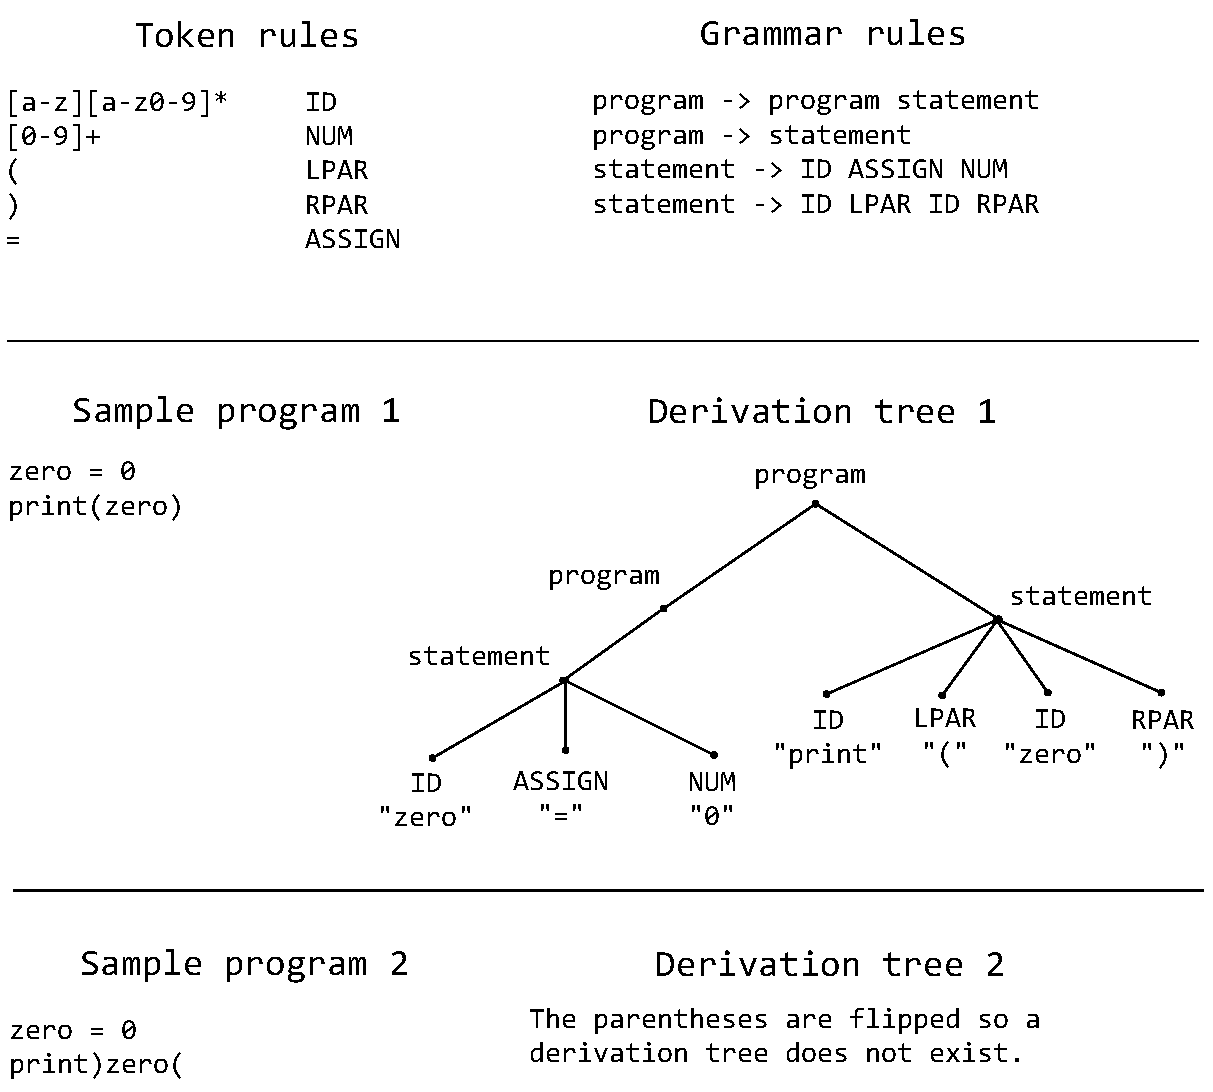
\includegraphics[width=\textwidth]{../img/tokens_and_grammar}
	\caption{Sample language definition with examples}
	\label{fig:chap1:tokens_and_grammar}
\end{figure}

On the figure \ref{fig:chap1:tokens_and_grammar} we see a set of token rules and grammar rules defining a~simple
language. Sample program $1$ shows a valid program in this language with its respective derivation tree, while
the second program does not adhere to the defined grammar rules.
Even tough this example is trivial it shows how vast majority of programming languages are processed:
\begin{itemize}
\item Lexical analysis splits the source code into tokens.
\item Syntax analysis builds a tree based on the grammar rules. This tree is typically called an AST\footnote{Abstract Syntax Tree} tree
and is similar to the derivation tree from the example.
\item AST is used to compile, interpret or transpile the source code.
\end{itemize}

Tokens do not have to consist of plaintext necessarily. Plaintext characters can be substituted with
images, videos, sounds, etc. In this thesis we construct a programming language with characters and some
of the tokens substituted with images or short looping videos (e.g. GIFs\footnote{Graphics Interchange Format is an image format that allows animations.}).
Figure \ref{fig:chap1:giflang_code} below shows the Sample program 1 from Figure \ref{fig:chap1:tokens_and_grammar} written in Giflang\footnote{We named the
programming language developed in this thesis Giflang}.
\begin{figure}[!hbt]
	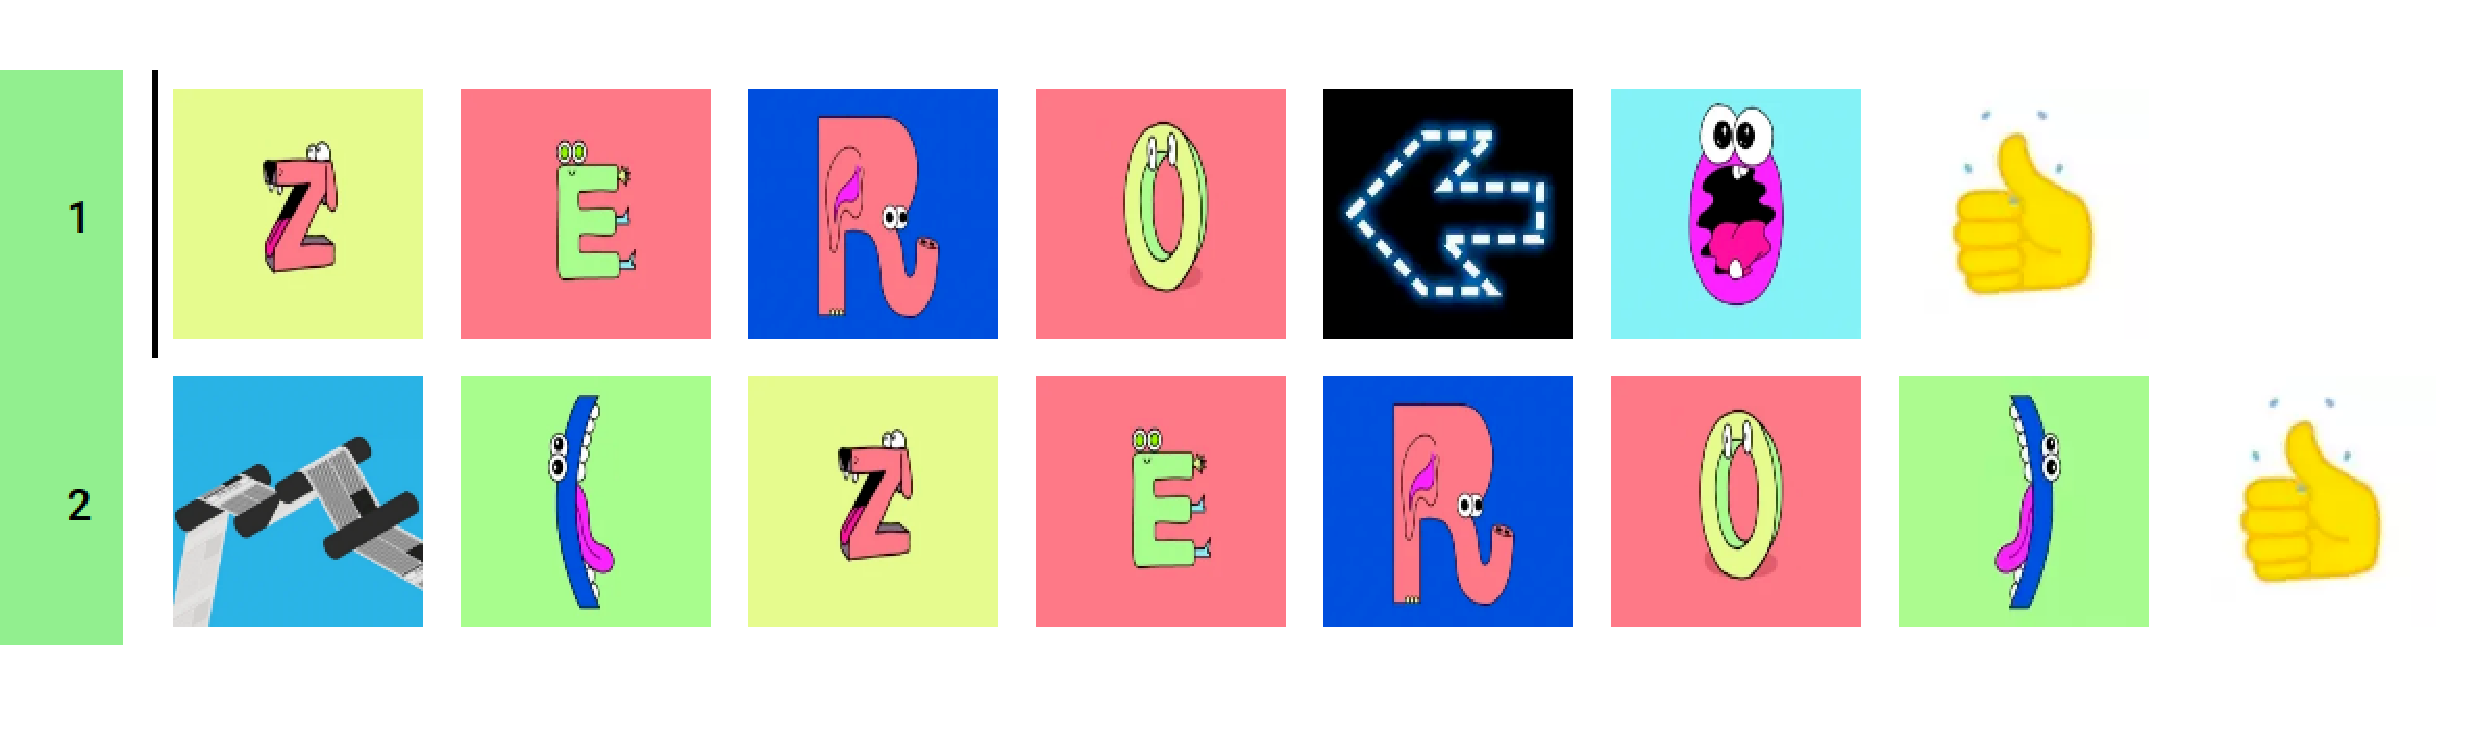
\includegraphics[width=\textwidth]{../img/giflang_code}
	\caption{Sample code in Giflang}
	\label{fig:chap1:giflang_code}
\end{figure}

You can see that characters and digits have their counterparts in Giflang. Assignment is represented with an arrow,
thumbs up is a semicolon and `print' function is a single image containing paper. The exact choice of images used here is of course
irrelevant.

In order to be able to store and parse programs like that we also need to define an intermediate
format. The format can be for example textual and the sample program from Figure \ref{fig:chap1:giflang_code} can be written as:
\begin{code}
Z;E;R;O; ASSIGN; 0; SEMICOLON;
PRINT; LPAR; Z;E;R;O; RPAR; SEMICOLON;
\end{code}

We actually chose to use a format very similar to the one above. We discuss the intermediate format and the language design
in section /TODO/.

You can see that there is a clear mapping between images and semicolon-delimited tokens. Therefore, a byproduct of
this thesis is a token-level programming language, i.e. a language that consists of delimited tokens. This tokens
can have different presentational forms as mentioned before.

A language like this one is of course impractical and hard to follow. We do not intend to create a language
for practical use. Our $3$ main motivations for creating Giflang are:
\begin{enumerate}
\item An image-based programming language like this does not exist yet. We show similar projects in Section \ref{chap1:related_work}. 
\item Using it in programming camps for elementary and high schoolers. We co-organize a Computer Science competition
named Prask \cite{Prask}. After each semester we invite best contestants to a week-long programming camp
filled with creative games mostly related to Computer Science. We plan on incorporating Giflang into the games.
\item Allowing users to substitute images for their own can give younger users feeling of creating ''their own language''.
\end{enumerate}

Since we use images instead of characters we need to implement our own IDE\footnote{Integrated Development Environment} to be able to
create and run Giflang programs.

To sum up it up, in this thesis we design a programming language with characters and some of the tokens substituted for images.
Additionally, we build an interpreter and an IDE for this language that both run in browser. Goals mentioned here are described
more precisely in the Section \ref{chap1:thesis_goals}. 

\section{Related work}
\label{chap1:related_work}
Visual programming languages are commonly used to introduce young audience to programming and this thesis was undeniably inspired by them. A visual 
programming language lets users create programs by manipulating program elements graphically rather than by specifying them textually\footnote{Wikipedia}.
Giflang is not a visual programming language as users can not manipulate with graphical objects in its IDE, e.g. move it or connect it with other
objects. It is also not a textual language per se as text is replaced by images. However, it is definitely closer to a textual than
a visual programming language.

\subsection{Emojicode}
An excerpt from the official documentation says that Emojicode \cite{Emojicode} is an open source, high-level, multi-paradigm programming language consisting of emojis.
It features Object-Orientation, Optionals, Generics and Closures.

Below is a `Hello World' program written in Emojicode:
\begin{figure}[!hbt]
	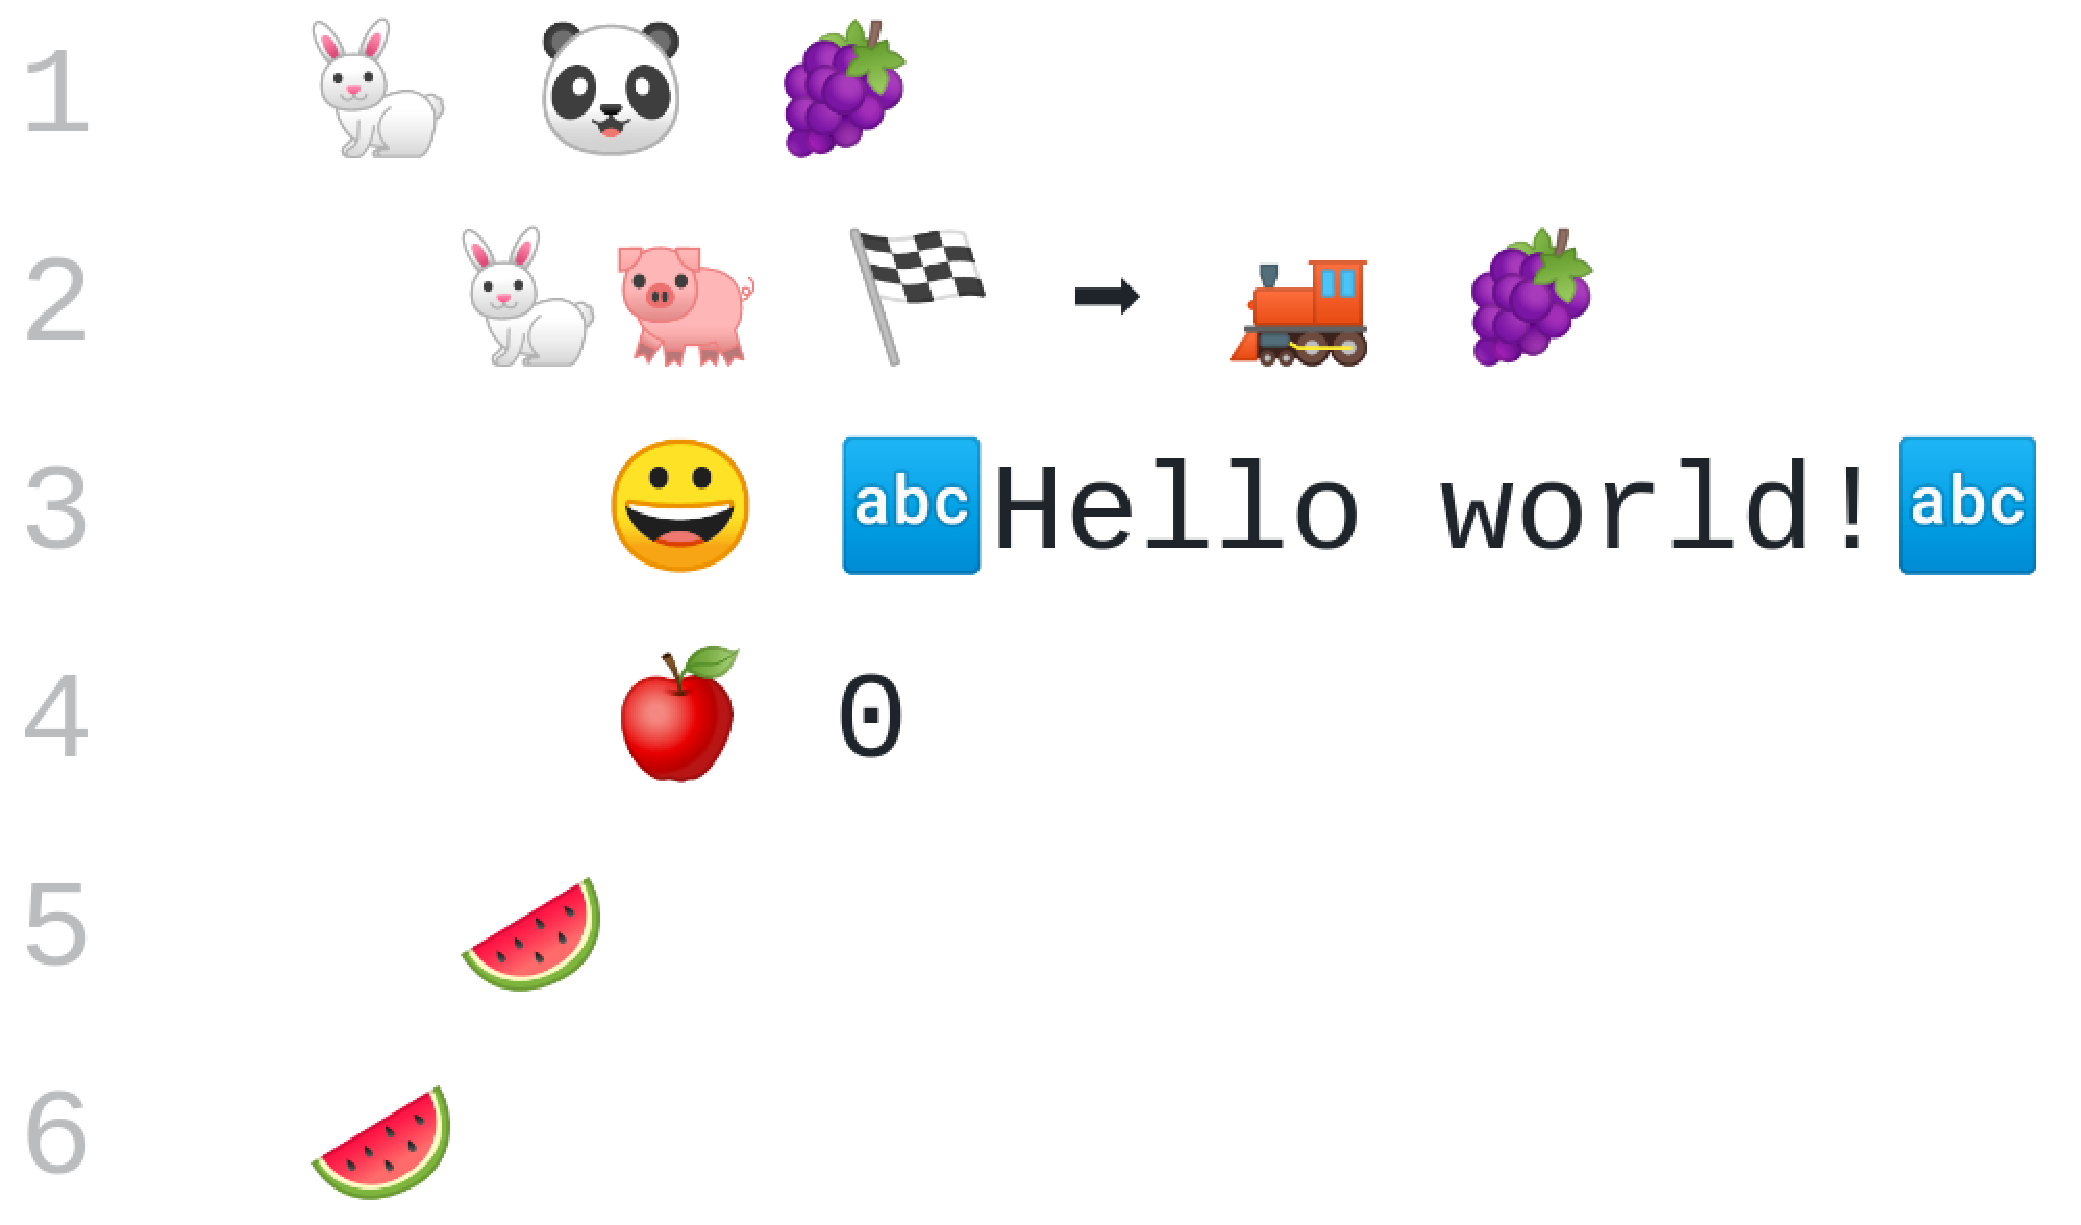
\includegraphics[width=0.5\textwidth]{../img/emojicode_helloworld}
	\label{fig:chap1:emojicode_helloworld}
\end{figure}

All built-in keywords and most of the special characters are replaced by emojis. For example a raspberry is an opening curly brace `{' in Emojicode.
However, as you can see in the `Hello World' program not every character is replaced by an emoji. Additionally, users can not create their own emoji
mappings to keywords or characters. Creating Emojicode sources is simple as emojis are just Unicode characters and most of the modern text editors
have a good support for them.

Source code is compiled first to LLVM IR\footnote{IR or Intermediate Language is a low-level programming language similar to assembly.} and then to
machine code. With features such as compilation to an intermediate language, object-orientation, static typing and garbage collection we can
say that Emojicode is similar to languages like C\# or Java.

Emojicode is similar to the language we build in this thesis. However, since we are replacing characters and keywords with arbitrary images as
opposed to emojis we have to use an intermediate textual format that maps to the images. Emojicode does not have this problem since emojis are
Unicode characters that can be represented in plaintext and parsed.

\subsection{JSFiddle}
JSFiddle \cite{JSFiddle} is a web IDE for testing and showcasing user-created and collaborational HTML, CSS and JavaScript code snippets, known as
'fiddles'\footnote{wikipedia copypaste}.

\begin{figure}[!hbt]
    \centering
	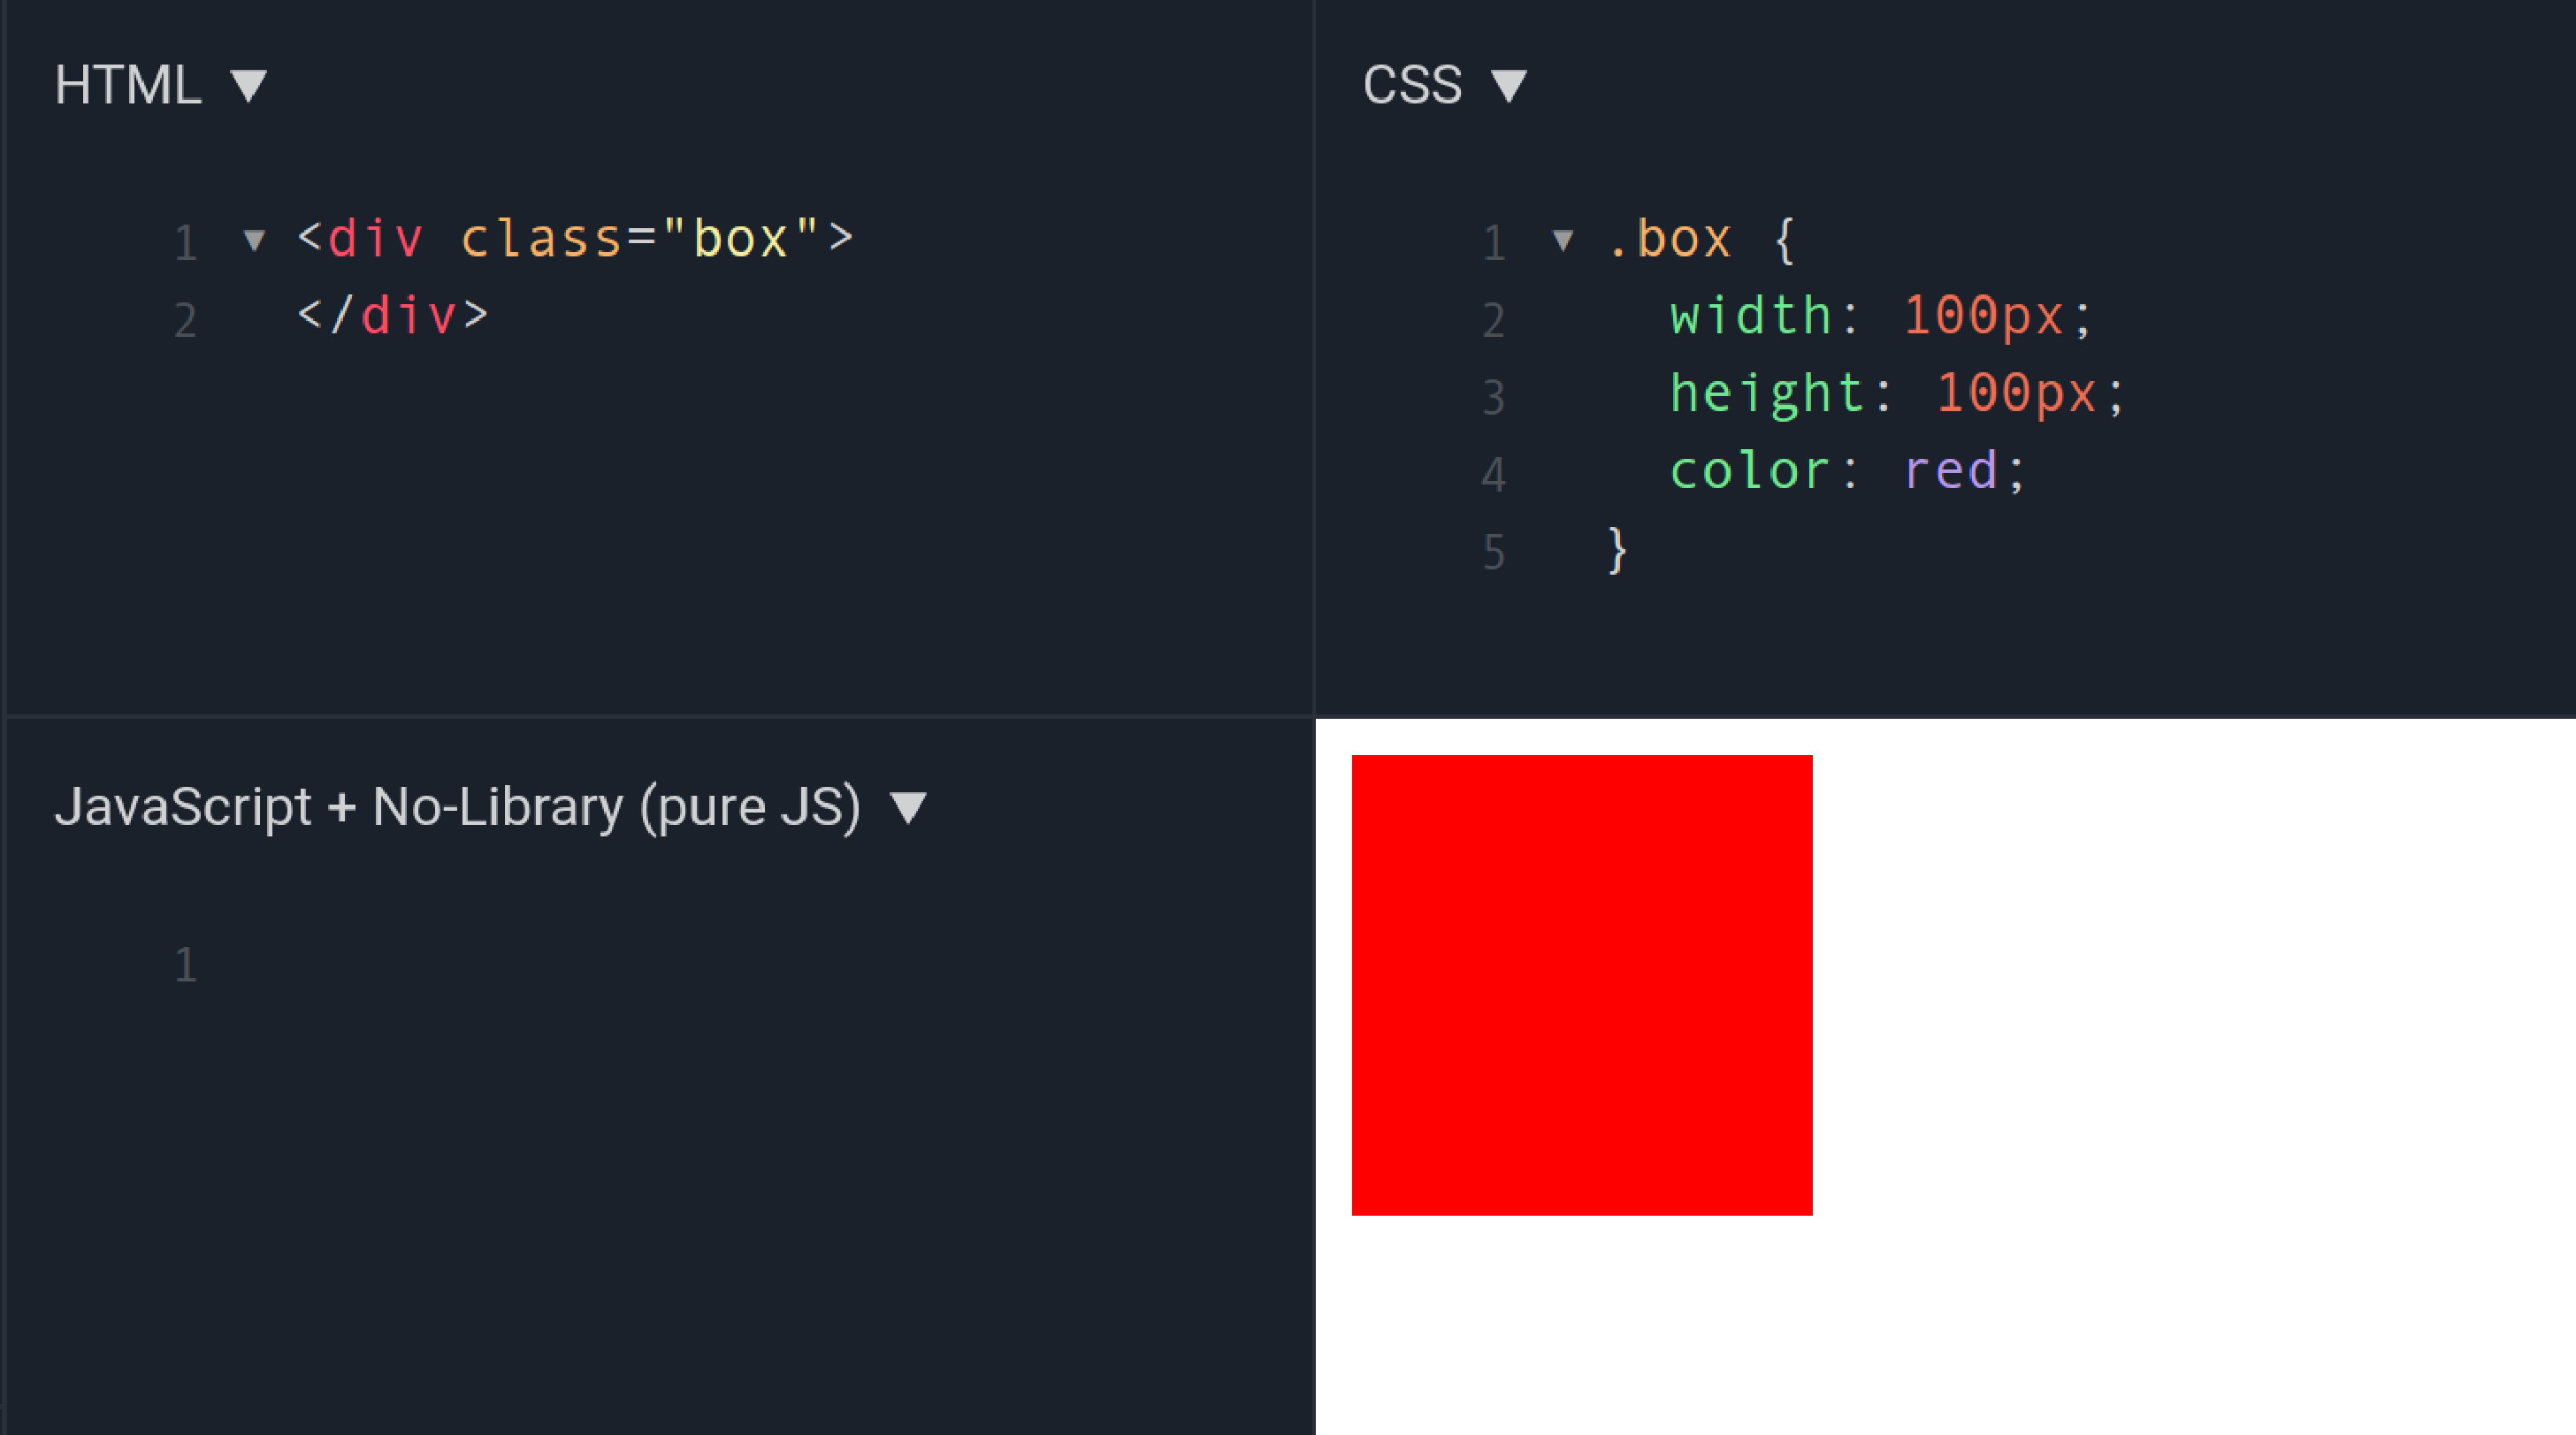
\includegraphics[width=\textwidth]{../img/jsfiddle}
	\caption{Sample fiddle}
	\label{fig:chap1:jsfiddle}
\end{figure}

In Figure \ref{fig:chap1:jsfiddle} you can see the main part of its UI. Users can input HTML, CSS and JavaScript and the output is displayed in the
bottom right quadrant.

JSFiddle offers an interesting way of storing and forking\footnote{Forking an existing project means creating a new project based on the existing one.}
fiddles. Firstly, user opens a URL that contains an ID of a fiddle that should be loaded. Afterwards user can edit the sources and run the fiddle.
At this point the edited fiddle is not stored on the server. It is only stored after explicitly saving it. The save action gives current fiddle a new ID.
This is how an existing fiddle can be forked. Any subsequent saves to the fork result in a  new 'revision' number that is also appended to the URL.

Revisions are numbered with natural numbers starting at 1. Each fiddle can be viewed at any of its revision numbers. In Figure \ref{fig:chap1:jsfiddle_url}
below you can see a URL with both an ID and a revision number.
\begin{figure}[!hbt]
    \centering
	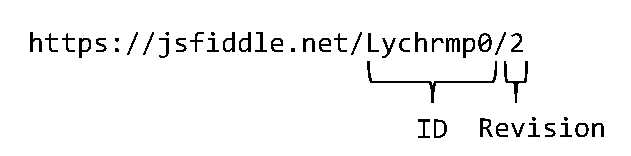
\includegraphics[width=0.5\textwidth]{../img/jsfiddle_url}
	\caption{JSFiddle URL}
	\label{fig:chap1:jsfiddle_url}
\end{figure}

We got inspired by this simple storing and forking design and as mentioned in the section \ref{chap2:program_id} we use a similar approach in the Giflang IDE.

JSFiddle executes user code on the client side since all of the input languages (HTML, CSS, JavaScript) are natively supported in browsers.

\section{Thesis goals}
\label{chap1:thesis_goals}
In this section we define the scope of the thesis and formulate its precise goals. Primarily, we want to build an image-based programming language
with characters and keywords substituted with images. Since we want to make it easily accessible for users we want to implement its
IDE as a web application.

We can split the goals into three major parts shown in the list below. We define goals separately for every part:
\begin{enumerate}
\item Giflang language design
   \begin{enumerate}[label=(\alph*)]
     \item Choose a suitable language type (Object-Oriented, functional, \ldots)
	 \item Define syntax, semantics and basic standard library
   \end{enumerate}
\item Client-side Interpreter
   \begin{enumerate}[label=(\alph*)]
	 \item Design and implement an interpreter for Giflang
	 \item Support code stepping with information about current position in the source code, call stack and environment
	 \item Implement an API for standard I/O\footnote{I/O stands for input and output.}
   \end{enumerate}
\item Web IDE
   \begin{enumerate}[label=(\alph*)]
     \item Design and implement an editor with characters replaced by images and support basic editing operations such as Delete,
     Backspace or moving with arrows
	 \item Allow specifying input to a running program and showing its output using images
	 \item Support code stepping with visualizations of currently executed position in the source code
	 \item Allow storing current program on the server and loading a previously saved program
	 \item Allow changing images in the mapping of images to characters and keywords
	\end{enumerate}
\end{enumerate}

Since the language is not meant for an actual app development we do not impose any performance goals on the interpreter. Rather than that we focus on features
like code stepping with highlighted source position.

\chapter{Moving to the Web}
\label{chap2}

We decided to build Giflang's interpreter and the IDE for web and we tried to move as much code to the client side as possible, resulting in a server that
simply serves static files. This chapter sheds light on why we decided to do so.

We believe that the usage of web browsers compared to other desktop apps is very high.\footnote{We did not
find any statistics backing up this statement. /TODO: Try harder/} Google is even building an operating system called ChromeOS based around their
market-dominating browser Chrome. With modern Web APIs, apps that were previously thought of as typical desktop apps are now moving to the browser. Below
are a few examples of such apps:
\begin{enumerate}
\item Photopea \cite{Photopea} -- A Photoshop web alternative
\item Google Hangouts \cite{Hangouts} -- A pioneer WebRTC\footnote{WebRTC (Web Real-Time Communication) provides web browser 
applications with real-time communication (RTC) via simple APIs.} app providing realtime video communication
\item TODO: Add an in-browser FPS here
\end{enumerate}

\section{Native vs Web IDE}
Most well known IDEs (e.g., Visual Studio, Eclipse or Xcode) are desktop applications. Web IDEs such as REPL.it or Ideone, on the other hand,
are not very widespread. We think that this is because users usually want to edit local files while browsers have limited support for reading
and saving local files programmatically. There is no Web API to overwrite a file at a given location on a user's disk for example.
Browsers prohibit this to protect the user's security.

Giflang is not suited for use in any serious project development and it is also not intended for such use. It is meant for creating
challenging and fun environment for solving programming problems. Standard I/O can be used for accepting problem inputs and writing results.

Therefore, Giflang does not have to support file I/O, multi-source programs and other otherwise-standard functionality. Of course later
on a graphical output, file I/O or other features can be added, but within the scope of this thesis we only plan on supporting
basic functionality.

Considering the above paragraphs we concluded that web IDE is more suitable for our type of application since it offers benefits as
ease of access and installation-free setup. In our opinion this outweighs the advantages of desktop IDEs such as easy local disk
file access and higher performance.

\section{Client side vs server side interpreter}

The Giflang code can be either interpreted on the server side or client side. By server side we mean any code that runs on the server. This means that
the interpret could be written in almost any language using any technologies, because it is up to us to choose what we run on the server. On the other hand,
client side code is executed in the browser which can only run JavaScript or WebAssembly.

\subsection{Server side execution}
Executing code on the server side means that in order to interact with it (e.g., provide interactive input or see gradual output) browser and
server need to communicate during the execution. There are $2$ basic approaches to this communication:
\begin{enumerate}
\item HTTP polling -- client (browser) initiates the communication to the server and waits for a response
\item WebSockets -- client and server open a two-way channel (WebSocket) through which the server can send messages to the client without
the client sending a request 
\end{enumerate}

\begin{figure}[!hbt]
	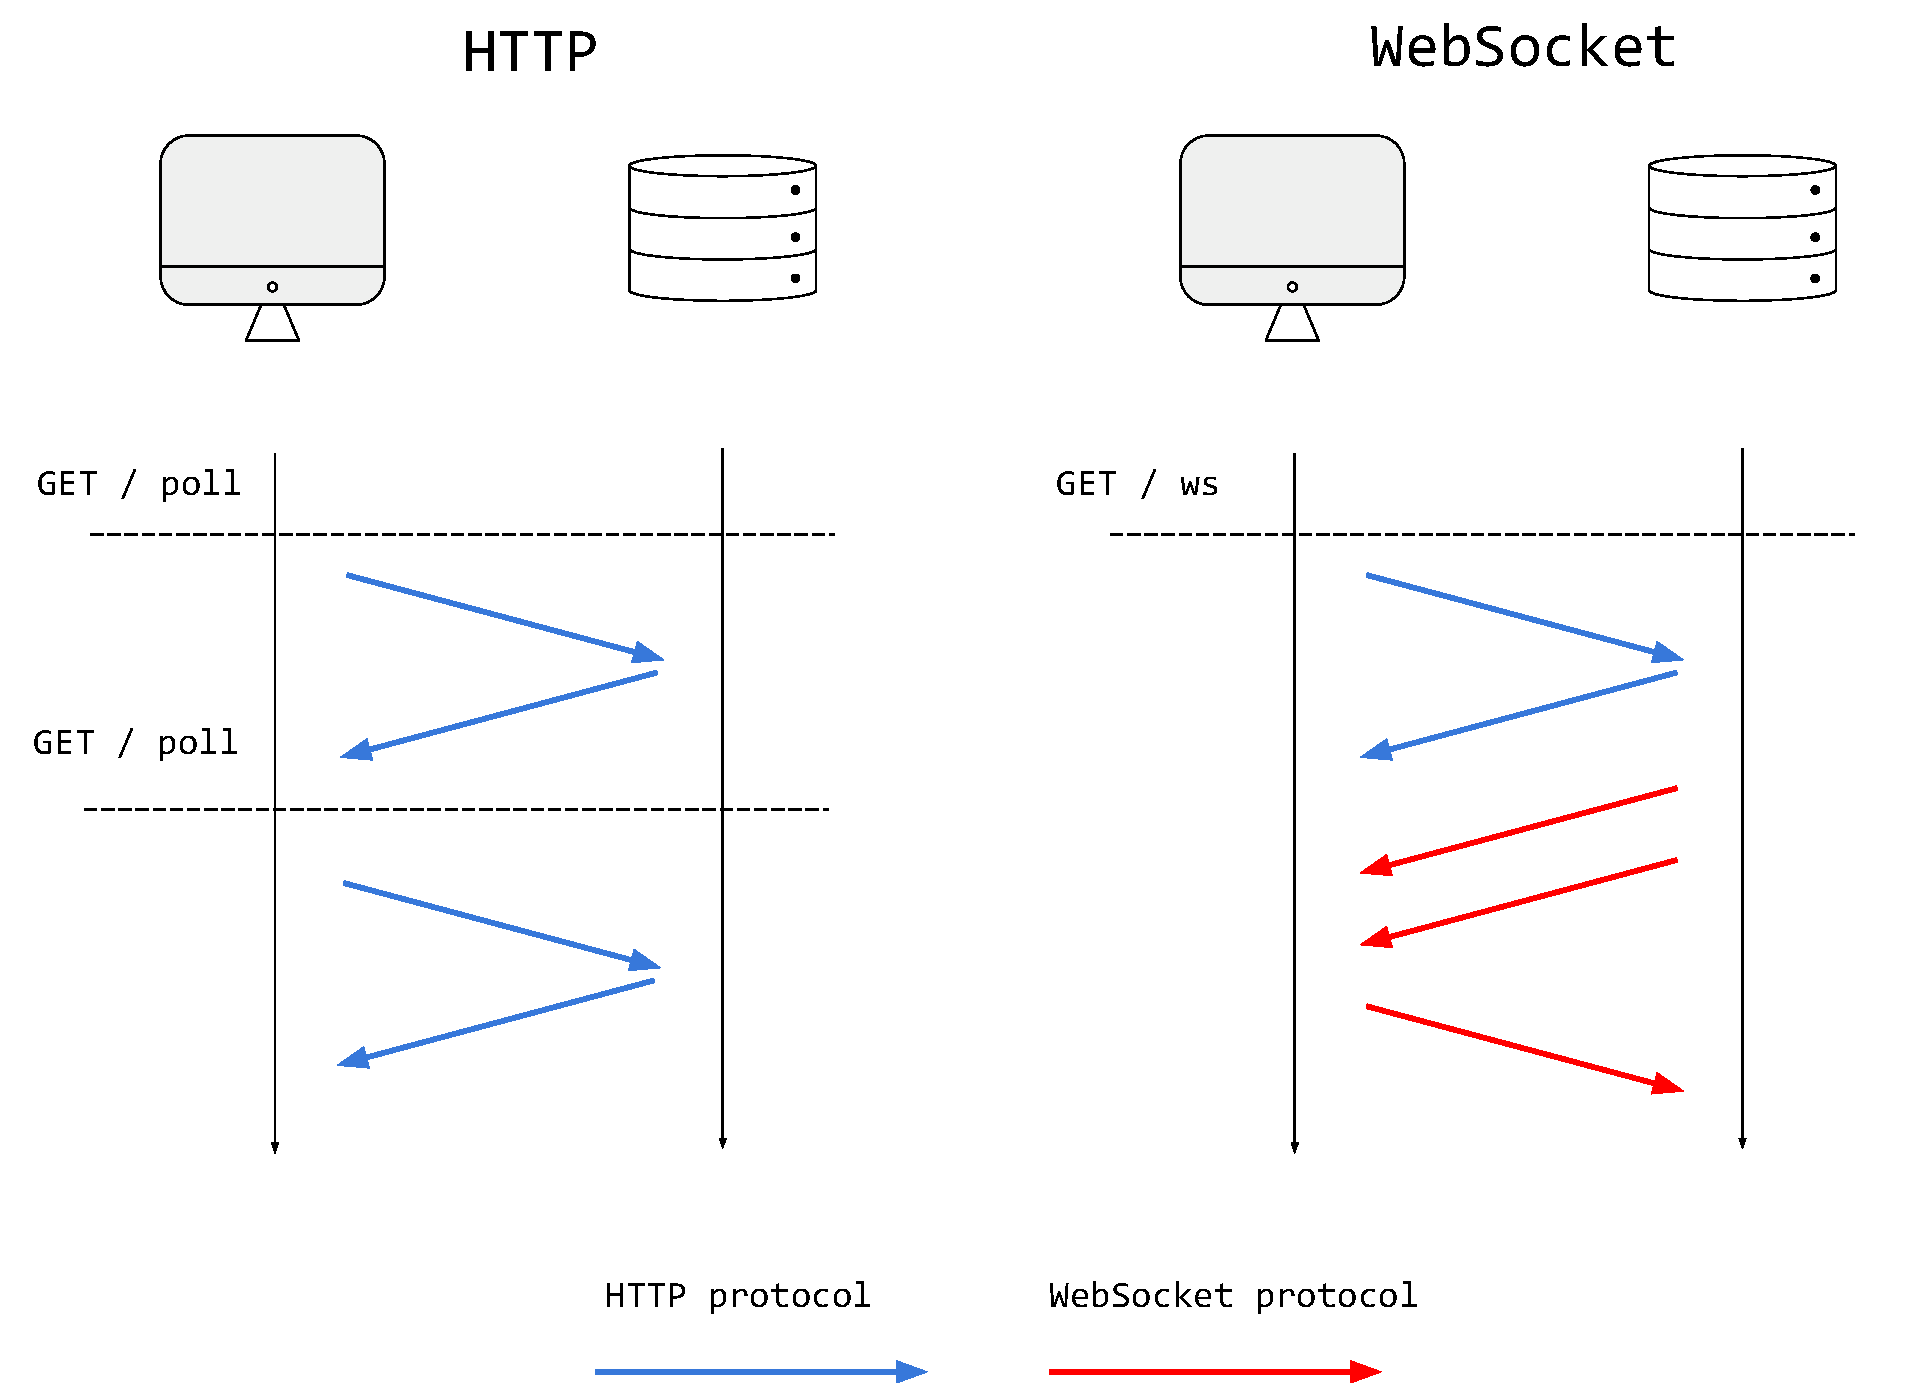
\includegraphics[width=\textwidth]{../img/websockets}
	\caption{Difference between using HTTP polling and WebSockets}
	\label{fig:chap2:websockets}
\end{figure}

We will introduce two Web IDEs that use server side execution -- REPL.it and Ideone. They both support numerous languages such
as Python, C, C++ and Java.

Ideone uses HTTP polling to get updates about the execution. Firstly, it sends a request to the backend containing source code and input.
After that it polls the server for an update every second. The server can respond with new output, error report, finish status, etc. Users of Ideone need to
specify all the output at once before the start. While it would be possible to implement interactive IO with the polling Ideone chose not to do so.
We did not find out why.

Having to poll the server for updates is awkward. If the granularity of polling is high requests are send frequently, but
in between consecutive requests the state might not have changed. That results in wasting resources. On the other hand, if the granularity is low less
requests are send, but that might result in higher latency between a state change happening on the server and the client picking it up.

WebSockets address this issue. They allow opening a two-way interactive communication session between the user's browser and a server.
With this API, browser can send messages to a server and receive event-driven responses without having to poll the server for a reply\footnote{source: mdn todo}.
You can see this in Figure \ref{fig:chap2:websockets} where WebSocket communication is marked with red arrows.
Before WebSockets were introduced around the year 2012 there was not a way to initiate a communication from server to browser as HTTP is a request-response
protocol. This means that server can only respond to browser's requests.

REPL.it is more modern compared to Ideone and uses WebSockets. It also provides interactive IO and debugging.

\subsection{Client side execution}
By default, the browser uses a single thread -- also called the main thread -- to run all the JavaScript in user's page, as well as to perform layout
changes, reflows, and garbage collection. As a result of this, long-running JavaScript functions can block the thread, leading to an unresponsive page and
a bad user experience.\footnote{source: mdn}

\subsubsection{WebWorkers}
Running the interpreter in the main thread would take processing time from UI updates which could lead to a bad responsiveness of the site. To
address this issue, browsers adopted support for WebWorkers. WebWorkers allow us to run scripts in the background threads, leaving main thread
to handle UI-related tasks.

Sharing data between threads is typically achieved by accessing the same piece of memory. However, communication between WebWorkers and the main
thread is achieved via messages:
\begin{code}
// Main script
var myWorker = new Worker('worker.js');
myWorker.postMessage('Hello Worker');

// worker.js
onmessage = function(msg) {
  console.log('Got a message from main: ' + msg);
}
\end{code}

An interpreter running in a separate WebWorker does not take processing time from the UI tasks in the main thread. We could not find an existing
project that would interpret or compile code in a WebWorker.

\subsubsection{WebAssembly}
JavaScript in the browser is executed by a JavaScript engine. Different browsers might have different engines. As Figure \ref{fig:chap2:v8_bench} shows,
JavaScript engines like V8 or SpiderMonkey keep improving in terms of speed. Nonetheless, a program written in a language
with highly optimized compiler like C++ or Rust that compiles to machine code will most probably outperform any JavaScript engine.

\begin{figure}[!hbt]
	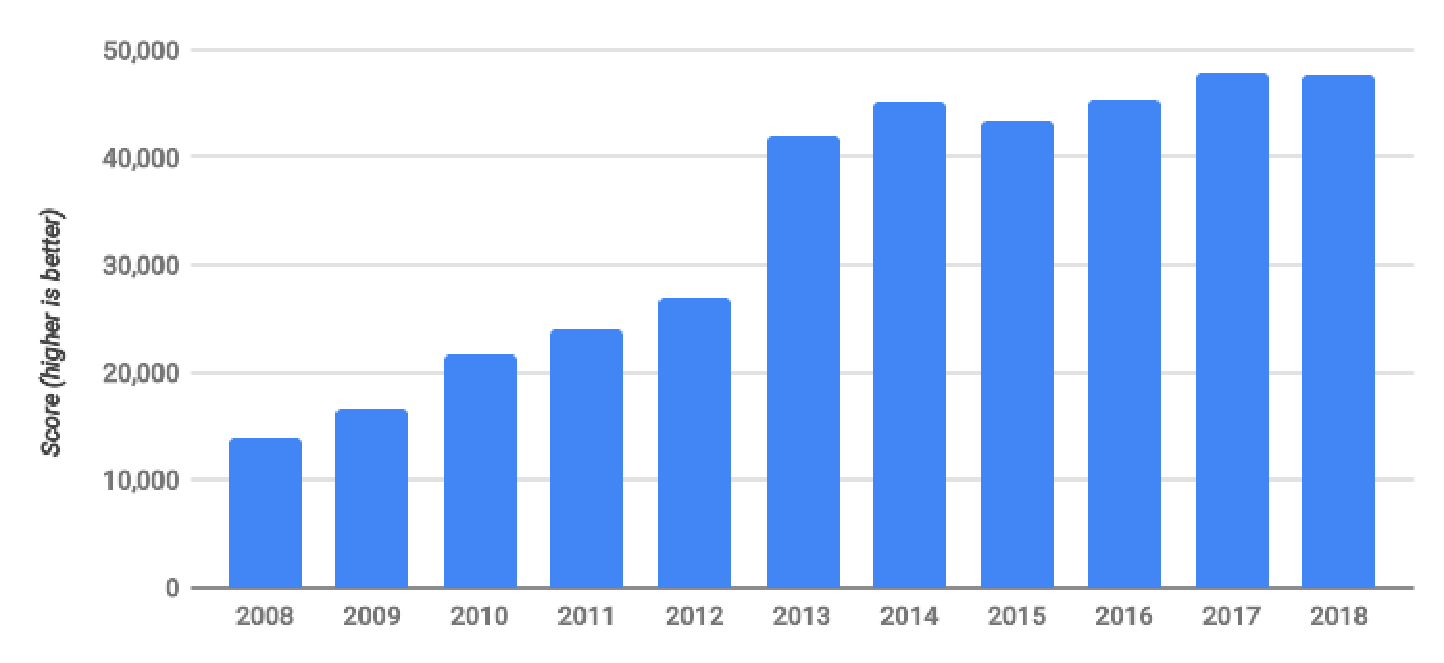
\includegraphics[width=\textwidth]{../img/v8-bench}
	\caption{A chart showing V8 improving over the years. Source: \href{https://v8.dev/blog/10-years}{v8.dev}}
	\label{fig:chap2:v8_bench}
\end{figure}

In order to close the gap between computational-heavy programs executing well natively while poorly in browser, WebAssembly
language was introduced in 2015. WebAssembly is a low level language that is now supported by all major browsers. Since it is
close to machine code, it is meant to be a compilation target language of other higher level languages.

Currently, many languages such as C/C++, Rust or TypeScript, can be compiled to WebAssembly. These compilers typically also emit
a `glue code' that contains handles that allow calling functions defined in the WebAssembly code from JavaScript.

Integrating functions defined in WebAssembly into a JavaScript script requires non-trivial effort since only primitive types can be passed
as function arguments and return values.

There are many ports of existing interpreters and compilers to WebAssembly, because there are tools like Emscripten\footnote{Add reference}
that can compile C/C++ code to WebAssembly. For example we really like Iodide\footnote{Todo reference} -- project that brings scientific Python
to the client side of the browser.

\subsection{Conclusion}
The advantage of server side interpreter is speed as the interpreter can use almost any technology. Web IDEs typically choose
server side execution for different reason, though. It is simpler than implementing interpreters for given languages in JavaScript or
porting the existing interpreters to WebAssembly. Since in our project we do not care so much about execution speed and
we do not have an existing interpreter or compiler, we can do better than server side execution.

The client side execution requires no special support from the server and it also works offline, i.e., after user looses connection. Running an interpreter
compiled to WebAssembly in a WebWorker would be the best approach as it would provide performance and also offloading from the main thread.
However, when we started working on the thesis we did not have any prior experience with writing an interpreter and adding another layer into the stack in the
form of WebAssembly seemed very complex. It would allow us to use language like C++ or Rust for the development, though. To keep things simpler we
decided to write the interpreter in JavaScript and run it in a WebWorker.

\section{Picking the right Javascript flavour}
JavaScript started evolving again in 2015, when a new standard -- ECMAScript 2015 -- was published. Prior to that, the last prominent
standard was introduced in 2009. Currently, there is a new standard released every year. With all the new additions to the language, programming in
JavaScript nowadays is way more pleasant than ever before.

However, it is still a dynamically typed language. Since we prefer statically typed languages we looked into the options of writing client-side scripts in
a statically typed language. It seems like every Silicon Valley tech giant tried to bring types to JavaSript. Google created Dart,
Facebook made Flow and finally, Microsoft created TypeScript. All of these languages can be transpiled to JavaScript while enforcing the static types.

Dart is a Java-like programming language, quite far from JavaScript in terms of its syntax. Flow is not a programming language in itself. It lets programmers
annotate a JavaScript code with types and enforce them. TypeScript is similar to Flow, but it is more popular and has a bigger community.

Among the languages described above we picked TypeScript, mainly because it has currently a lot of momentum and it is being widely adopted.

\section{The rise of single-page applications}
In the old days of the web, before the year 2000, any data exchange between a server and a browser required reloading an entire page. 
Ajax\footnote{Asynchronous JavaScript + XML} was introduced to solve this problem by allowing web applications to send and retrieve data from
a server asynchronously (in the background) without interfering with the display and behavior of the existing page\footnote{wikipedia}.

Ajax later gave rise to single-page applications (SPAs). SPA is a web application that interacts with the user by dynamically rewriting
the current page rather than loading entire new pages from a server\footnote{wikipedia}. In this thesis, we build an SPA, because users should not
face any page-reloads while interacting with a web IDE (e.g., when running or saving the code).  

Browsers were originally designed for a stateless page-redraw model and thus with SPAs some new challenges emerged. The most predominant of them is
probably keeping the displayed UI in sync with the state.

Let us show what we mean by keeping the state in sync with the UI on a simple example. Consider a widget for creating a list of emails like one shown below.
Users can add emails and delete them later. This example is inspired by the one shown in the article \cite{JSFramework}.
\begin{figure}[!hbt]
    \centering
	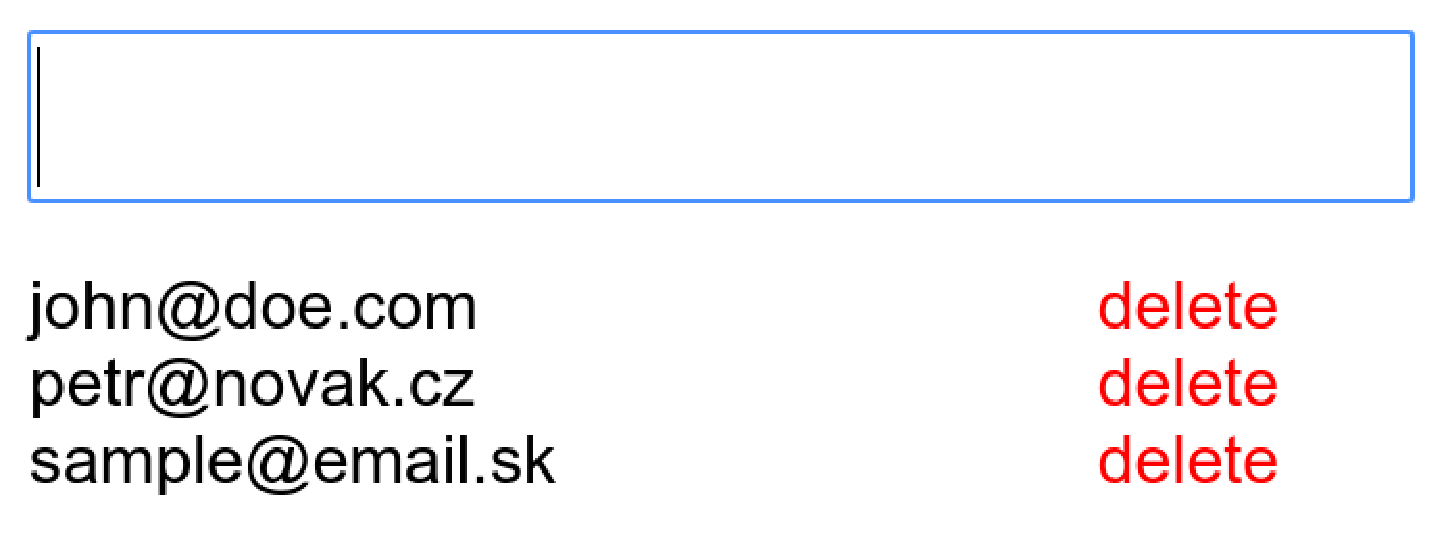
\includegraphics[width=0.5\textwidth]{../img/emails}
	\caption{A simple widget for creating a list of emails}
	\label{fig:chap2:emails}
\end{figure}

We can represent the state of this application as a list of emails with a unique ID. Below is a JavaScript object holding the state displayed in
Figure \ref{fig:chap2:emails}.
\begin{code}
let state = [
    { email: 'john@doe.com', id: 0 },
    { email: 'petr@novak.cz', id: 1 },
    { email: 'sample@email.sk', id: 2 },
]
\end{code}

Every user action that changes the state has to also update the UI accordingly. For example adding an email must add it to the state object, but also update
the DOM\footnote{The Document Object Model (DOM) is a programming interface for HTML and XML documents.} by appending a new element to the email list.
Similarly, removing an email should remove it from the list and from the UI.
\begin{code}
// DOM nodes of the list.
let li_items = []
// List of emails with IDs.
let state = []

function addEmail(email) {
    // State change
    const id = GetNextId()
    state = state.concat({ email, id })

    // UI change
    const ul = document.createElement('ul')
    const li = document.createElement('li')
    const span = document.createElement('span')
    const del = document.createElement('a')
    span.innerText = email
    del.innerText = 'delete'
    del.setAttribute('data-delete-id', id)

    ul.appendChild(li)
    li.appendChild(del)
    li.appendChild(span)
    li_items[id] = li
}

function removeEmail(id) {
    // State change
    state = state.filter(item => item.id !== id)

    // UI change
    const ul = document.createElement('ul')
    ul.removeChild(li_items[id])
}
\end{code}

This example is very basic, but for more complex apps with bigger states, it is very easy to end up with the UI and the state out of sync. It is the case
because we have to write code for both the state change and the UI change. On the other hand, JavaScript frameworks abstract away the fact that UI needs
to be updated accordingly when the state changes. They simply give a guarantee that whenever the state is mutated, the UI gets updated.

\subsection{React}
React \cite{React} is a JavaScript framework created by Facebook. To make sure the UI corresponds to the state, the whole UI is re-rendered
when the state changes. However, re-renders are costly operations and deleting the whole DOM and creating a new one from scratch on every re-render
would be very slow. Instead, React renders the page into a Virtual DOM. Virtual DOM is a “virtual” representation of a UI kept in memory and
synced with the “real” DOM by React\footnote{React docs}. This process is called reconciliation.

The reconciliation takes the current virtual DOM and a snapshot of the last synced virtual DOM and tries to find the minimum number of operations to turn
one into another. There are some generic solutions to this algorithmic problem of generating the minimum number of operations to transform one tree into another.
However, the state-of-the-art algorithms \cite{TreeEditDistance} have a complexity in the order of $\mathcal{O}(n^3)$ where $n$ is the number of elements in
the tree\footnote{taken from React docs}. Therefore, React team decided to implement a heuristic $\mathcal{O}(n)$ algorithm.

\begin{figure}[!hbt]
    \centering
	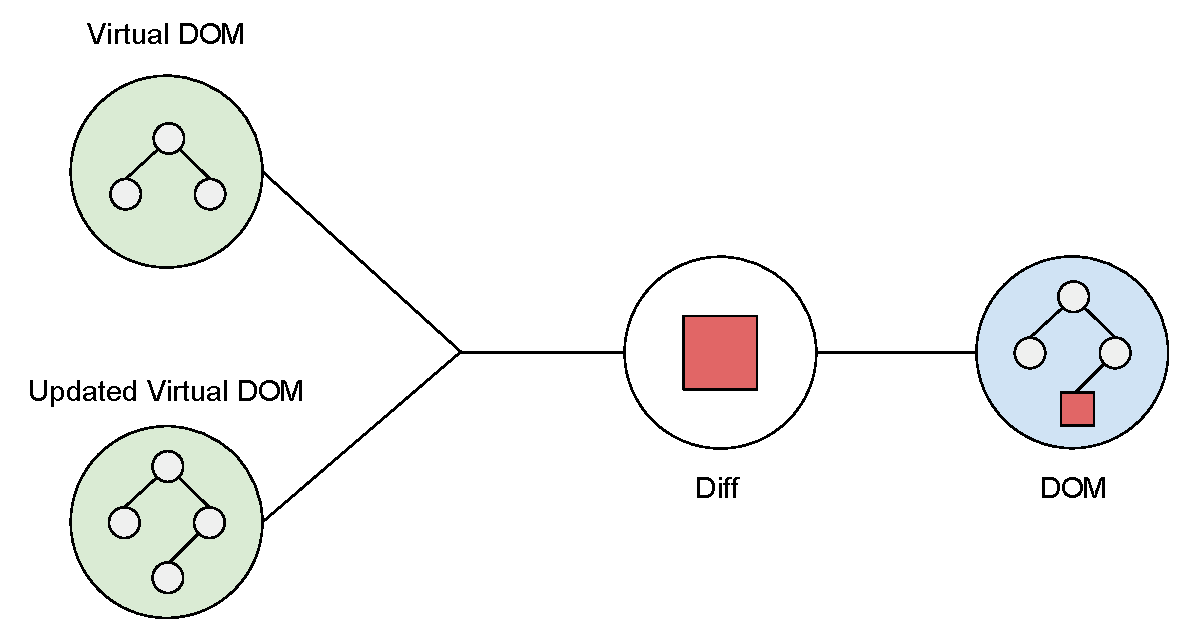
\includegraphics[width=\textwidth]{../img/virtual_dom}
	\caption{A flowchart of React updating the DOM.}
	\label{fig:chap2:virtual_dom}
\end{figure}

There are many other frameworks (e.g., Angular, Vue.js, Ember.js). Each of them has a different approach to solving the UI and the state syncing. However, we picked
React for this project, mainly because we used it in previous projects where it proved itself very useful and easy to use.

\section{Storing programs}
We want to allow users to save, load and share their programs. A typical solution to this problem is to create a database in the backend. However, since all
of our application logic lies on the client side we looked into a way of opting out of creating a database and using a ready-made service. This means that
our backend can consist of only a server serving static files.

\subsection{Backend as a service}
Backend as a service (BaaS) is a model for providing app developers with a way to link their applications to backend cloud storage and APIs exposed by back end
applications while also providing features such as user management or push notification.\footnote{wikipedia} These services are provided via the use of custom
SDKs\footnote{Software development kit} and APIs.

There are many different BaaS providers (e.g., Back4App, Parse Server or AWS Aurora), but we chose to use Firebase /TODO cite/ from Google. Since we do not
need a complex functionality for our project, picking almost any other provider would still work well with our app.

The biggest advantage of BaaS over a custom backend is that BaaS saves developers a lot of time as it typically offers user management and data storage.
Providers usually promise seamless scaling of the app. On the other hand, BaaS gives developers less control as they have to adhere to the limits of the APIs
and it can also cost more than a VPS with a custom server.

\subsection{Sharing and forking the programs}
\label{chap2:program_id}

In order to allow users sharing their programs with other users, we need to give each program a unique ID which can then be used to load the program later.
This ID can be put in the URL for example as a GET parameter or part of the path.

When a user program is saved for the first time, it is given a unique ID. Any subsequent saves overwrite the current version. If we keep overwriting
a saved program even after a page reload, user A might load a program of user B and overwrite the work of user B.

In order to prevent users from overwriting each others' programs, we decided to always assign a new ID to a program that is saved for the first time after
a page load. This allows users to fork an existing program without having an ability to change it.

\begin{figure}[!hbt]
    \centering
    \begin{tikzpicture}[scale=0.2]
    \tikzstyle{every node}+=[inner sep=0pt]
    \draw [black] (21.4,-32.1) circle (3);
    \draw (21.4,-32.1) node {$S$};
    \draw [black] (45.6,-32.1) circle (3);
    \draw (45.6,-32.1) node {$id$};
    \draw [black] (67.6,-32.1) circle (3);
    \draw (67.6,-32.1) node {$newId$};
    \draw [black] (24.4,-32.1) -- (42.6,-32.1);
    \fill [black] (42.6,-32.1) -- (41.8,-31.6) -- (41.8,-32.6);
    \draw (33.5,-32.6) node [below] {Page\mbox{ }load\mbox{ }/id};
    \draw [black] (46.923,-34.78) arc (54:-234:2.25);
    \draw (45.6,-39.35) node [below] {Edits};
    \fill [black] (44.28,-34.78) -- (43.4,-35.13) -- (44.21,-35.72);
    \draw [black] (48.6,-32.1) -- (64.6,-32.1);
    \fill [black] (64.6,-32.1) -- (63.8,-31.6) -- (63.8,-32.6);
    \draw (56.6,-32.6) node [below] {First\mbox{ }save};
    \draw [black] (68.923,-34.78) arc (54:-234:2.25);
    \draw (67.6,-39.35) node [below] {Edits\mbox{ }and\mbox{ }saves};
    \fill [black] (66.28,-34.78) -- (65.4,-35.13) -- (66.21,-35.72);
    \end{tikzpicture}
	\caption{A state machine showing how program ID changes in the web IDE.}
	\label{fig:chap2:page_url}
\end{figure}

JSFiddle mentioned in the section \ref{chap1:related_work} uses the same approach. Additionally, JSFiddle also stores all intermediate versions. However,
we did not find it crucial and chose to overwrite the current version after each save, except for the initial save.


\chapter{Language design}
\label{chap3:language_design}

When creating Giflang we had two options:
\begin{enumerate}
    \item Use a language with an existing web interpreter
    \item Create a new language and a web interpreter
\end{enumerate}

In the first section of this chapter we explain why we decided to not reuse an existing language. Later, we discuss the design of our own language. We do not
precisely define all the semantics, but rather provide a high-level overview. We think that it is more important to explain \emph{why} Giflang uses specific
constructs, rather than show \emph{how} these constructs behave in every case.

The language documentation with examples can be found in the web IDE. /TODO: Where?/

\section{Reusing an existing interpreter}
In the previous Chapter \ref{chap2} we concluded that interpreting the user code on the client-side is the best option for our project. Therefore, when
looking for a language to reuse we need to limit ourselves to the ones that have an existing web interpreter, i.e., an interpreter written in either
JavaScript or WebAssembly. The two major languages that have existing web interpreters are Python and JavaScript.

\subsection{Python}
There are multiple Python web interpreters, for example Pyodide \cite{Pyodide} or Brython \cite{Brython}. Pyodide works by compiling CPython \cite{CPython}
to WebAssembly using Emscripten. On the other hand, Brython works by transpiling Python to JavaScript. We were not able to find a Python web interpreter that would
support code stepping out of the box. We considered forking either Pyodide or Brython and adding this functionality.

Adding code stepping to Pyodide would require changing the underlying CPython implementation. CPython is very complex and was not built for this use case.
On the other hand, Brython is fully written in JavaScript and also builds an AST from a Python code in JavaScript. There
is a fork of Brython \cite{PythonDebugger} that implements code stepping. However, at closer inspection we found out it runs the code all at once and records trace information
at each executed line by inserting a trace function call there. Afterwards, it only gives the user an illusion of code stepping.

It is possible to create a ``live'' code stepping for Brython in a similar fashion, for example with the aid of Atomics API discussed in /TODO section/.
We did not find a simple way of increasing the stepping granularity from just lines to arbitrary AST nodes, though. We definitely could have adjusted Brython instead
of creating a custom interpreter. However, it would take a non-trivial effort to change the Brython's internals and we rather put this effort into creating
a new interpreter from scratch and learning a lot about languages and interpreters along the way.

\subsection{JavaScript}
There are numerous JavaScript interpreters written in JavaScript. The one closest to our needs is JS-Interpreter \cite{JSInterpreter} that supports running JavaScript
with code stepping in isolation. It was designed for use in Blockly \cite{Blockly}, a library for building visual programming editors.

JS-Interpreter supports only ES5\footnote{ECMAScript 5 or ECMAScript 2009} standard of JavaScript. This standard has no \texttt{class} keyword or block-scoped
variables with \texttt{let} keyword. We find ES5 way of defining classes using functions and prototypes confusing:
\begin{code}
// ES 5
function Person(name) {
    this.name = name;  
}

Person.prototype.greet = function () {
    console.log('Hello my name is ' + this.name);
}

// ES 6
class Person {
    constructor(name) {
        this.name = name
    }

    greet() {
        console.log('Hello my name is ' + this.name);
    }
}
\end{code}

We could add support for ES6 features to the JS-Interpreter and use it for our project. However, as in the case of Brython we decided to rather put the effort into
creating a new solution than putting a lot of effort an existing one.

\section{Text format}
Before we dive into the language itself, let us first discuss the text representation of the language. Since it is intended for being displayed in
graphics using images, we considered defining the language in terms of semicolon delimited tokens where each token can be substituted with a single image.
Below is an identity function defined in both a \emph{character-level} and a \emph{token-level format}.
\begin{code}
// Token-level
FUNCTION; I;D; LPAR; A; RPAR; LCURLY;
RETURN; A; SEMICOLON;
RCURLY;

I;D; LPAR; 8; RPAR; SEMICOLON;

// Character-level
function ID(A) {
    return A;
}

ID(8);
\end{code}

We could just replace all characters of the character-level format with images, but keywords like \texttt{function} would result in multiple images. In the token-level
format we define function as a single token \texttt{FUNCTION} and is thus replaced with a single image.

In case of the character-level format, we could replace everything character by character with images unless \texttt{function} or any other keyword is found in which
case we would replace it with a single image. However, there are some cases to keep an eye on; for example we should consider:
\begin{itemize}
    \item An identifier \texttt{functionA} should not have its \texttt{function} part replaced for an image.
    \item When an image for a keyword, e.g., \texttt{function} is used inside a string, it should be represented as a single character.
\end{itemize}

Another option is to represent keywords as single characters in the character-level format. This makes the image substitution trivial, as we can substitute
every character. The ``keyword characters'' have to be unique among other characters. To illustrate this, we can use a Unicode letter `f' with a hook $f$
to represent a function and a character $\hookleftarrow$ for return.
\begin{code}
$f$ ID(A) {
    $\hookleftarrow$ A;
}

ID(8);
\end{code}

The above approach that uses Unicode characters has a nice property regarding the use of the keywords in a string. According to the ECMAScript specification,
Section 8.4/TODO cite/: \emph{When a String contains actual textual data, each element is considered to be a single UTF-16 code unit.} This means that if we
only use characters that can be encoded into a single 16-bit code unit, all keywords will take space of a single character in a string.

At first we implemented the token-level format approach. It made the implementation of the parser harder, as typical lexer responsibilities like processing
an identifier had to be moved to the syntactical analysis. Later on, we decided to switch to the character-level format with keywords substituted for
Unicode characters. We change the format mostly because we realized that the token-level format only introduced more complexity with no real benefits.

\section{Deciding on a language type}
Since we have chosen to build our own language it is time to decide on what kind of language it should be and what features it should have. There are
multiple types of programming languages and we will briefly go through the most known ones.

\subsection{Functional programming}
Functional programming treats computation as the evaluation of mathematical functions and avoids changing-state and mutable data.\footnote{wikipedia}
This means that functional programming languages do not support imperative flow controls like loop statements, conditional statements like if-else and
switch statements.

On the other hand, pure functions are very typical for functional programming. \emph{Pure functions} are functions whose outcome depends solely on their arguments
and create no side-effects (e.g., by changing a global variable). Eliminating side effects can make understanding a program easier, which is one of the
key motivations for the development of functional programming.\footnote{wiki}

Additionally, functional programming often relies on recursion and functions being first-class entities. Being a first-class entity means that functions can appear
anywhere in the program where other first-class entities like numbers can, including arguments to other functions and their return values.

One of the typical examples of a functional programming language is Haskell. It was created in 1990, it is statically typed, supports type inference,
and lazy evaluation. Below is a sample program in Haskell finding the edit distance\footnote{} between two strings from the official docs.
\begin{code}
import Data.Array as Array

editDistance :: Eq a => [a] -> [a] -> Int
editDistance xs ys = table ! (m,n)
    where
    (m,n) = (length xs, length ys)
    x     = array (1,m) (zip [1..] xs)
    y     = array (1,n) (zip [1..] ys)
    
    table :: Array (Int,Int) Int
    table = array bnds [(ij, dist ij) | ij <- range bnds]
    bnds  = ((0,0),(m,n))
    
    dist (0,j) = j
    dist (i,0) = i
    dist (i,j) = minimum [table ! (i-1,j) + 1, table ! (i,j-1) + 1,
        if x ! i == y ! j
            then table ! (i-1,j-1)
            else 1 + table ! (i-1,j-1)]
\end{code}

\subsection{Object-oriented programing}
Object-oriented programming (OOP) is based around the concept of ``objects'' which can contain data, in the form of fields (also known as attributes or properties),
and code, in the form of methods.\footnote{wiki} Object's methods can access and modify the object they are operating on using a keyword like \texttt{this}
or \texttt{self}.
Programs are then made out of objects that interact together.

The most popular OOP languages are class-based (e.g., C++, Java, Python), meaning that objects are instances of classes, which also determine their types.\footnote{wiki}
There are also alternatives, for example JavaScript is prototype-based.

OOP has a few features that are common among most of the object-oriented programming languages:
\begin{itemize}
    \item Inheritance or subclassing lets developers create a new class by building upon an existing one.
    \item Encapsulation allows hiding data and methods of an object from the outside interference and misuse.
    \item Polymorphism allows calling code to be agnostic as to which class in the supported hierarchy it is operating on.
\end{itemize}

Below is an example of polymorphism in C++.
\begin{code}
class Animal {
public:
    Animal() : { }
    virtual string make_sound() = 0;
};

class Dog: public Animal {
public:
    Dog() : Animal() { }
      
    string make_sound() { 
        return "Woof, woof!"; 
    }
};

class Sheep: public Animal {
public:
    Sheep() : Animal() { }
      
    string make_sound() { 
        return "Baa, baa!"; 
    }
};

int main() {
    Animal *animal;
    Dog dog();
    Sheep sheep();

    // Store the address of Dog.
    animal = &dog;

    // Call Dog's make_sound. Returns "Woof, woof!".
    animal->make_sound();

    // A similar example with sheep. Returns "Baa, baa!".
    animal = &sheep;
    animal->make_sound();

    return 0;
}
\end{code}

\subsection{Esoteric programming languages}
An esoteric programming language is designed to experiment with weird ideas, to be hard to program in, or as a joke, rather than for practical use. We can not
describe esoteric languages in general as they all use different ideas.

Probably the most popular esoteric language is brainf***. It operates on an array of memory cells, also referred to as the tape. All of the cells are initially
set to zero. There is a single pointer, initially pointing to the first memory cell. The language has the following commands:

\begin{figure}[!hbt]
    \centering
    \begin{tabular}{|c l |} 
    \hline
    $>$ & Move the pointer to the right \\
    \hline
    $<$ & Move the pointer to the left \\
    \hline
    $+$ & Increment the memory cell under the pointer \\
    \hline
    $-$ & Decrement the memory cell under the pointer \\
    \hline
    $.$ & Output the character signified by the cell at the pointer \\
    \hline
    $,$ & Input a character and store it in the cell at the pointer \\
    \hline
    $[$ & Jump past the matching ] if the cell under the pointer is 0 \\
    \hline
    $]$ & Jump back to the matching [ if the cell under the pointer is nonzero \\
    \hline
    \end{tabular}
    \caption{A list of brainf*** commands}
\end{figure}

Other examples of esoteric languages are:
\begin{itemize}
    \item Shakespeare /TODO ref/, a programming language whose source code resembles Shakespeare plays. 
    \item Befunge /TODO ref/, a language where the code is layed out on a two-dimensional grid of instructions, and execution can proceed in any direction of that grid.
\end{itemize}

\subsection{Conclusion}
There are also other programming language types apart from the ones mentioned here, for example logic programming. We did not plan on using
concepts from these languages and therefore we did not list them. It would be great to combine a language presented in images with an esoteric language
of some sort. However, we did not come up with an interesting enough model and we did not want to blindly reuse an existing one. In the end we settled on
a more conservative approach.

Since our intended audience is typically experienced in Python we decided to base our language around "Pythonic" features. We also think
the class-based model of Python is more intuitive than prototype-based one found for example in JavaScript.

Even though the author of this thesis likes statically-typed languages, Giflang is dynamically-typed. The primary reason is that images take a lot of
space on the user screen and hence we tried to keep the language concise. Adding typed declarations would probably make it less error-prone, but more verbose.

\section{Object model}
As mentioned in the end of the previous section we base Giflang on Python. Everything is an object in Python. We will now explain in more detail what exactly
it means. An object \texttt{A} can have multiple related objects:
\begin{itemize}
    \item An object \texttt{B} that denotes the type of \texttt{A}. We call \texttt{B} \emph{a klass} of the instance \texttt{A} and we say that \texttt{A}
    is an instance of \texttt{B}.
    \item If \texttt{A} is a class it can have multiple \emph{base classes}. Let \texttt{B} denote one of the base classes. We say that \texttt{A}
    \emph{derives from} \texttt{B}. 
\end{itemize}

Since classes are objects, they have to be instances of \emph{some} class. We call this ``class of classes'' a \texttt{MetaClass}. Now of course
\texttt{MetaClass} is also an object and thus has to be an instance of \emph{some} class. To break the chain, \texttt{MetaClass} is an instance of itself.
Figure \ref{fig:chap3:python_structure} describes the Python's object structure in more detail.

\begin{figure}[!hbt]
    \centering
    \tikzset{every picture/.style={line width=0.75pt}} %set default line width to 0.75pt        
    \trimbox{0cm .75cm 0cm 0cm}{
        \begin{tikzpicture}[x=0.75pt,y=0.75pt,yscale=-1,xscale=1]
        \draw   (13.61,159.25) -- (125.73,159.25) -- (125.73,200.19) -- (13.61,200.19) -- cycle ;
        \draw    (67.11,199.26) .. controls (87.27,268.92) and (-12.63,252.81) .. (12.38,202.52) ;
        \draw [shift={(13.61,200.19)}, rotate = 479.36] [fill={rgb, 255:red, 0; green, 0; blue, 0 }  ][line width=0.08]  [draw opacity=0] (10.72,-5.15) -- (0,0) -- (10.72,5.15) -- (7.12,0) -- cycle    ;
        \draw   (14.54,80.16) -- (126.66,80.16) -- (126.66,121.1) -- (14.54,121.1) -- cycle ;
        \draw  [dash pattern={on 0.84pt off 2.51pt}]  (58.73,160.18) -- (58.73,129.48) -- (58.73,125.03) ;
        \draw [shift={(58.73,122.03)}, rotate = 450] [fill={rgb, 255:red, 0; green, 0; blue, 0 }  ][line width=0.08]  [draw opacity=0] (10.72,-5.15) -- (0,0) -- (10.72,5.15) -- (7.12,0) -- cycle    ;
        \draw   (14.54,2) -- (126.66,2) -- (126.66,42.94) -- (14.54,42.94) -- cycle ;
        \draw  [dash pattern={on 0.84pt off 2.51pt}]  (68.97,80.16) -- (68.97,49.45) -- (68.97,45.01) ;
        \draw [shift={(68.97,42.01)}, rotate = 450] [fill={rgb, 255:red, 0; green, 0; blue, 0 }  ][line width=0.08]  [draw opacity=0] (10.72,-5.15) -- (0,0) -- (10.72,5.15) -- (7.12,0) -- cycle    ;
        \draw    (82,122.03) -- (82,155.32) ;
        \draw [shift={(82,158.32)}, rotate = 270] [fill={rgb, 255:red, 0; green, 0; blue, 0 }  ][line width=0.08]  [draw opacity=0] (10.72,-5.15) -- (0,0) -- (10.72,5.15) -- (7.12,0) -- cycle    ;
        \draw   (163.41,159.25) -- (275.54,159.25) -- (275.54,200.19) -- (163.41,200.19) -- cycle ;
        \draw    (162.95,179.72) -- (129.66,179.72) ;
        \draw [shift={(126.66,179.72)}, rotate = 360] [fill={rgb, 255:red, 0; green, 0; blue, 0 }  ][line width=0.08]  [draw opacity=0] (10.72,-5.15) -- (0,0) -- (10.72,5.15) -- (7.12,0) -- cycle    ;
        \draw  [dash pattern={on 0.84pt off 2.51pt}]  (216.45,159.25) -- (130.12,104.11) ;
        \draw [shift={(127.59,102.49)}, rotate = 392.57] [fill={rgb, 255:red, 0; green, 0; blue, 0 }  ][line width=0.08]  [draw opacity=0] (10.72,-5.15) -- (0,0) -- (10.72,5.15) -- (7.12,0) -- cycle    ;
        \draw   (313.22,149.02) -- (425.35,149.02) -- (425.35,209.5) -- (313.22,209.5) -- cycle ;
        \draw    (312.76,179.72) -- (279.47,179.72) ;
        \draw [shift={(276.47,179.72)}, rotate = 360] [fill={rgb, 255:red, 0; green, 0; blue, 0 }  ][line width=0.08]  [draw opacity=0] (10.72,-5.15) -- (0,0) -- (10.72,5.15) -- (7.12,0) -- cycle    ;
        \draw    (286.5,26.74) -- (223.15,26.74) ;
        \draw [shift={(220.15,26.74)}, rotate = 360] [fill={rgb, 255:red, 0; green, 0; blue, 0 }  ][line width=0.08]  [draw opacity=0] (10.72,-5.15) -- (0,0) -- (10.72,5.15) -- (7.12,0) -- cycle    ;
        \draw  [dash pattern={on 0.84pt off 2.51pt}]  (286.5,60.74) -- (223.15,60.74) ;
        \draw [shift={(220.15,60.74)}, rotate = 360] [fill={rgb, 255:red, 0; green, 0; blue, 0 }  ][line width=0.08]  [draw opacity=0] (10.72,-5.15) -- (0,0) -- (10.72,5.15) -- (7.12,0) -- cycle    ;
        \draw (69.67,179.72) node   [align=left] {{\fontfamily{pcr}\selectfont MetaClass}};
        \draw (70.6,100.63) node   [align=left] {{\fontfamily{pcr}\selectfont ObjectClass}};
        \draw (70.6,23.4) node   [align=left] {{\fontfamily{pcr}\selectfont NULL}};
        \draw (219.48,179.72) node   [align=left] {{\fontfamily{pcr}\selectfont UserClass}};
        \draw (370.87,179.72) node   [align=left] {{\fontfamily{pcr}\selectfont  UserClass}\\{\fontfamily{pcr}\selectfont instance}};
        \draw (351.87,25.72) node   [align=left] {{\fontfamily{pcr}\selectfont Instance of}};
        \draw (357.87,60.72) node   [align=left] {{\fontfamily{pcr}\selectfont Derives from}};
        \end{tikzpicture}
    }
    \caption{Object structure in Python.}
	\label{fig:chap3:python_structure}
\end{figure}

\texttt{MetaClass} is actually called \texttt{type} in Python. Below is an interactive Python session that unveils the internals of Python shown in the
Figure \ref{fig:chap3:python_structure}.
\begin{code}
>>> class X:
...     pass
... 
>>> type(X)
<class 'type'>
>>> x = X()
>>> type(x)
<class '__main__.X'>
>>> x.__bases__
Traceback (most recent call last):
  File "<stdin>", line 1, in <module>
AttributeError: 'X' object has no attribute '__bases__'
>>> type(type(X))
<class 'type'>
>>> type(X).__bases__
(<class 'object'>,)
>>> type(type(X).__bases__[0])
<class 'type'>
\end{code}

We decided to reuse this model as the base of Giflang.

\subsection{Magic Methods}
Another Python feature we reused are magic methods. They provide a very straightforward way
to overload operators. Magic methods are prefixed and suffixed with two underscores. Below is a Python example that uses magic methods:
\begin{code}
class Number:
    # Defines a constructor
    def __init__(self, val):
        self.val = val
    
    # Defines a string representation
    def __str__(self):
        return str(self.val)

    # Overloads operator +
    def __add__(self, other):
        return Number(self.val + other.val)

    # Overloads a call operator
    def __call__(self):
        return 'An instance was called :)'

x = Number(2)
y = Number(3)
# Outputs 5. First __add__ is called and then __str__ on the result.
print(x + y)
# Outputs 'An instance was called :)'
print(x())
\end{code}

The example shows how to create a constructor, overload an operator and create a new instance of a class by calling the class with arguments for the constructor.
\texttt{Number} class also defines a \texttt{\_\_call\_\_} method so naturally we might expect the call \texttt{Number(2)} to result in the string
`An instance was called :)'. However, it is not the case. Instead, \texttt{Number(2)} results in a new instance of the texttt{Number} class. The author of this
thesis thinks that this is the reason why magic method resolution in Python starts from the instance type rather than from the instance itself, as it is
the case with regular methods.

Following up on the idea from the previous paragraph, because the call \texttt{Number(2)} does not result in the call of the \texttt{\_\_call\_\_} function on the
\texttt{Number} type, it has to result in a \texttt{\_\_call\_\_} method further up the chain. In this case, \texttt{Number} is an instance of the \texttt{type},
or the \texttt{MetaClass} class. Its \texttt{\_\_call\_\_} method is responsible for creating a new instance and calling the \texttt{\_\_init\_\_} method. Oversimplified,
the \texttt{type}'s \texttt{\_\_call\_\_} function might look like this:
\begin{code}
class type:
    # Since classes are instances of the 'type' class, self
    # in this method is a class object. 
    def __call__(self, *args, **kwargs):
        obj = instantiate(self)
        obj.__init__(*args, **kwargs)
        return obj
\end{code}

In reality, creating a new instance is a little more complicated, To give users more control over the instantiation, another magic method (\texttt{\_\_new\_\_})
is called instead of a made up function \texttt{instantiate} in the example above. We will not go into more details since we decided not to include the
\texttt{\_\_new\_\_} magic method into Giflang as it is mainly used only for a few specific use cases (e.g., creating a singleton).

Having a keyword for introducing new variables, e.g., \texttt{var}, would mean that magic methods could be resolved the same way as normal methods. However,
we like the simplicity of creating a new instance via calling a class and hence used this approach in Giflang as well.

\section{Basic types}
There are 7 basic types supported natively in Giflang:
\begin{itemize}
    \item Object
    \item Number
    \item Boolean
    \item None
    \item Function
    \item List
    \item String
\end{itemize}

Since the interpreter is written in JavaScript, we based the types mostly around JavaScript types. For example, \texttt{Number} is a wrapper of the JavaScript
\texttt{number}. Because of this, it has a standard double-precision 64-bit floating point format (IEEE 754). Boolean \texttt{True} and \texttt{False}
and also \texttt{None} are all represented using a single image. In the language itself they are just global variables, similar to Python.

Functions are first-class entities, which means that users can create anonymous functions, pass callbacks, etc. Closures are also supported.
Lists and strings are basically wrappers around JavaScript arrays and strings as it was the simplest approach. There are no primitive types and everything is an
\texttt{Object}. Of course, it would be more effective to implement the \texttt{Number} as a primitive type, but as stated earlier, performance was not one of the main
objectives and implementing the \texttt{Number} as an \texttt{Object} was easier.

As with any other language there needs to be a support basic conversions. We could create explicit conversion functions, but since Giflang is dynamically typed, we can
implement conversions in the constructors of the target types. For example, calling \texttt{Number('1')} should result in a conversion from a \texttt{String} to
a \texttt{Number}.

\section{Flow constructs}
Giflang supports the following flow constructs: \texttt{if}, \texttt{while} and \texttt{for}. The author of this thesis is a fan of the C-like \texttt{for} and therefore
used it in Giflang as well. When evaluating a condition, a \texttt{\_\_bool\_\_} magic method is called on the resulting object to convert it to a boolean. By default,
everything except for \texttt{0}, \texttt{None}, \texttt{False}, an empty string and an empty list evaluates to \texttt{True}.

\section{Standard library}
Giflang's standard library is quite modest. There is only support for the very basics: \texttt{list}, \texttt{string}, \texttt{I/O}. As mentioned earlier, lists
and strings wrap standard JavaScript lists and strings. The I/O is provided in the form of three functions:
\begin{itemize}
    \item \texttt{input} function reads a single line
    \item \texttt{println} calls \texttt{\_\_str\_\_} magic method on its arguments to stringify them and outputs them on a single line adding a newline at the end
    \item \texttt{print} has the same semantics as \texttt{println}, but omits the newline at the end
\end{itemize}

We did not extend the library further since lists, strings, and I/O are the necessary building blocks that should suffice for most of the basic use-cases.
This thesis is quite broad in scope and the standard library of Giflang was one of the places where we cut a corner. Extending the library further would not
be hard, but we decided to invest the time into different areas of the project.
\chapter{Implementation}
In this chapter we describe implementation of Giflang and provide insights into the decisions we made along the way. As Figure \ref{fig:chap4:overview} shows,
the project consists of two major parts: an interpreter and a web IDE. These two components can be found in the \texttt{interpreter/} and the \texttt{frontend/}
folders, respectively. The Figure \ref{fig:chap4:overview} also outlines the API of the interpreter that allows the web IDE to execute user's programs.
This API is further discussed in subsection /TODO/
\begin{figure}[!hbt]
    \centering
    \label{fig:chap4:overview}
    \tikzset{every picture/.style={line width=0.75pt}} %set default line width to 0.75pt        
    \begin{tikzpicture}[x=0.75pt,y=0.75pt,yscale=-1,xscale=1]
    \draw   (37.5,92) -- (186.5,92) -- (186.5,228) -- (37.5,228) -- cycle ;
    \draw    (352.5,220) -- (189.5,220) ;
    \draw [shift={(186.5,220)}, rotate = 360] [fill={rgb, 255:red, 0; green, 0; blue, 0 }  ][line width=0.08]  [draw opacity=0] (10.72,-5.15) -- (0,0) -- (10.72,5.15) -- (7.12,0) -- cycle    ;
    \draw    (351.5,179) -- (189.5,179) ;
    \draw [shift={(186.5,179)}, rotate = 360] [fill={rgb, 255:red, 0; green, 0; blue, 0 }  ][line width=0.08]  [draw opacity=0] (10.72,-5.15) -- (0,0) -- (10.72,5.15) -- (7.12,0) -- cycle    ;
    \draw    (349.5,139) -- (185.5,139) ;
    \draw [shift={(352.5,139)}, rotate = 180] [fill={rgb, 255:red, 0; green, 0; blue, 0 }  ][line width=0.08]  [draw opacity=0] (10.72,-5.15) -- (0,0) -- (10.72,5.15) -- (7.12,0) -- cycle    ;
    \draw    (350.5,97) -- (188.5,97) ;
    \draw [shift={(185.5,97)}, rotate = 360] [fill={rgb, 255:red, 0; green, 0; blue, 0 }  ][line width=0.08]  [draw opacity=0] (10.72,-5.15) -- (0,0) -- (10.72,5.15) -- (7.12,0) -- cycle    ;
    \draw  [dash pattern={on 0.84pt off 2.51pt}]  (269,55.2) -- (269,91.2) ;
    \draw  [dash pattern={on 0.84pt off 2.51pt}]  (270,246.2) -- (270,264.2) ;
    \draw   (351.5,90) -- (500.5,90) -- (500.5,226) -- (351.5,226) -- cycle ;
    \draw (425,164) node   [align=left] {{\fontfamily{pcr}\selectfont IDE}};
    \draw (112.02,161) node   [align=left] {{\fontfamily{pcr}\selectfont Interpreter}};
    \draw (112.6,64.4) node  [font=\normalsize] [align=left] {{\fontfamily{pcr}\selectfont \textbf{WebWorker}}};
    \draw (425.6,64.4) node  [font=\normalsize] [align=left] {{\fontfamily{pcr}\selectfont \textbf{Main thread}}};
    \draw (276.02,232) node   [align=left] {{\fontfamily{pcr}\selectfont \textit{Execute code}}};
    \draw (273.02,194) node   [align=left] {{\fontfamily{pcr}\selectfont \textit{Next code step}}};
    \draw (272.02,152) node   [align=left] {{\fontfamily{pcr}\selectfont \textit{Get input}}};
    \draw (271.02,110) node   [align=left] {{\fontfamily{pcr}\selectfont \textit{Print output}}};
    \end{tikzpicture}
    \caption{A high-level diagram of the implementation}
\end{figure}

\section{Interpreter}
Every interpreter first \emph{parses} a source code and then \emph{executes} the parsed tree (Fig \ref{fig:chap4:interpreter}). There is a room for a lot of optimizations along the way in order
to make the execution as fast as possible. However, we do not incorporate any optimizations into the interpreter and only execute the parsed tree node by node.

\begin{figure}[!hbt]
    \centering
    \label{fig:chap4:interpreter}
    \tikzset{every picture/.style={line width=0.75pt}} %set default line width to 0.75pt        

    \begin{tikzpicture}[x=0.75pt,y=0.75pt,yscale=-1,xscale=1]
    %uncomment if require: \path (0,622); %set diagram left start at 0, and has height of 622

    %Shape: Rectangle [id:dp28122229657926034] 
    \draw   (226.5,34) -- (341.5,34) -- (341.5,110) -- (226.5,110) -- cycle ;
    %Straight Lines [id:da9888936135364137] 
    \draw    (411.25,72.5) -- (341.5,72.5) ;

    \draw [shift={(414.25,72.5)}, rotate = 180] [fill={rgb, 255:red, 0; green, 0; blue, 0 }  ][line width=0.08]  [draw opacity=0] (10.72,-5.15) -- (0,0) -- (10.72,5.15) -- (7.12,0) -- cycle    ;
    %Shape: Rectangle [id:dp7793277711435098] 
    \draw   (414.5,34) -- (606.5,34) -- (606.5,110) -- (414.5,110) -- cycle ;
    %Straight Lines [id:da7940866772557511] 
    \draw    (223.25,72.5) -- (89.85,72.5) ;
    \draw [shift={(87.5,72.5)}, rotate = 180] [color={rgb, 255:red, 0; green, 0; blue, 0 }  ][line width=0.75]      (0, 0) circle [x radius= 3.35, y radius= 3.35]   ;
    \draw [shift={(226.25,72.5)}, rotate = 180] [fill={rgb, 255:red, 0; green, 0; blue, 0 }  ][line width=0.08]  [draw opacity=0] (10.72,-5.15) -- (0,0) -- (10.72,5.15) -- (7.12,0) -- cycle    ;

    % Text Node
    \draw (283.5,61) node   [align=left] {{\fontfamily{pcr}\selectfont \textbf{Parsing}}};
    % Text Node
    \draw (510.5,57) node   [align=left] {{\fontfamily{pcr}\selectfont \textbf{Execution}}};
    % Text Node
    \draw (376.5,58) node   [align=left] {{\fontfamily{pcr}\selectfont \textit{AST}}};
    % Text Node
    \draw (284.5,85) node   [align=left] {{\fontfamily{pcr}\selectfont (Jison)}};
    % Text Node
    \draw (510.5,83) node   [align=left] {{\fontfamily{pcr}\selectfont (Visitor pattern)}};
    % Text Node
    \draw (156.5,57) node   [align=left] {{\fontfamily{pcr}\selectfont \textit{Source code}}};
    \end{tikzpicture}
    \caption{A diagram of the Giflang interpreter}
\end{figure}

\subsection{Parsing}
Parser is an interpreter component that checks whether the input source conforms to the rules of the formal grammar of a language. Additionally, parsers help
building an AST from the source code. In the very beginning of this thesis we briefly explained what grammar rules and AST is (see Fig \ref{fig:chap1:tokens_and_grammar})

Parsers usually consist of two separate parts: \emph{lexing} or \emph{tokenization} and \emph{parsing}. A lexer splits input text into \emph{tokens}.
For example it can split an input \texttt{'4 + size'} into following tokens:
\begin{code}
// Sample tokens for an input '4 + size'
[{ "Type": "NUMBER", "Text": "4" },
 { "Type": "OPERATOR", "Text": "+" },
 { "Type": "IDENTIFIER", "Text": "size" }]
\end{code}

Grammar rules are then defined in terms of tokens, for example:
\begin{figure}[!hbt]
\begin{code}
expression -> factor OPERATOR expression
expression -> factor
factor -> IDENTIFIER
factor -> NUMBER
\end{code}
    \caption{An example of a grammar definition}
    \label{fig:chap4:grammar}
\end{figure}

The grammar above defines a language consisting of expressions that can contain numbers and identifiers. It is very minimal as it does not account
for operator precedence or parenthesis. Lowercase words are \emph{nonterminals} and capitalized words are \emph{terminals}. Terminal symbols are elementary
symbols and can not be replaced by other terminals or nonterminals. Nonterminals can appear on the left side of productions and they are replaced by groups
of terminal symbols according to the production rules.

In order to parse a grammar like the one above, we can either create our own parser or use \emph{a parser generator}. We will briefly describe both options.
There are many ways of creating a custom parser, but we will discuss the most common one, a recursive-descent parser. Parsers are a large topic and
we do not intent to dive deep into it.

\subsubsection*{Recursive-descent parser}
A recursive-descent parser is a method of creating a parser using mutually recursive procedures where each procedure implements one of the nonterminals
of the grammar. To give us a better idea of what it means to create a function for each nonterminal, we created a parser for the grammar from
the Figure \ref{fig:chap4:grammar} in Python.
\begin{code}
# Unimplemented functions:
#   * curToken -- returns the current token
#   * nextToken -- advances to the next token

def accept(token):
    if curToken() == token:
        nextToken()
        return 1
    return 0

def expect(token):
    if accept(token):
        return 1
    raise Exception("expect: unexpected token")

def factor():
    if accept('IDENTIFIER'):
        # Action
        pass
    elif accept('NUMBER'):
        # Action
        pass 
    else:
        raise Exception("factor: syntax error")

def expression():
    factor()
    if accept('OPERATOR'):
        expression()
        # Action
        return
    # Action 
\end{code}

We can see that the grammar can be transformed into the code very naturally using a recursive-descent parser. The \texttt{'\# Action'} comments mark places where
grammar rules are applied and we could add bits of code there that would build a derivation tree.

Recursive-descent parsers can run in linear time with respect to the input string size, granted that the parsed grammar is an LL(k). \emph{An LL(k) grammar} is
a context-free grammar that is parsed by an LL parser, which parses the input from \textbf{L}eft to right and creates a \textbf{L}eftmost derivation.
Additionally, it requires at most $k$ lookahead tokens to uniquely identify which rule should be applied next.

\subsubsection*{Parser generators}
Creating parsers can be a repetitive process -- applying the same patterns to different grammars. Parser generators solve this by generating parsers from grammar
specifications. There are dozens of parser generators, but we will only describe one of them, GNU Bison/TODO cite/.

We will also use Flex in the examples, a lexical analyzer generator that is often used alongside Bison. Both Flex and Bison can target C, C++, and Java.

Flex takes token descriptions as regular expressions. The following code is not a valid Flex source, but it demonstrates the idea behind Flex:
\begin{code}
%{ %}

DIGIT           [0-9]
LETTER          [a-zA-Z]

%%
{DIGIT}+                        return NUMBER;
{LETTER}({LETTER}|{DIGIT})*     return IDENTIFIER;
[+-]                            return OPERATOR;
%%
\end{code}

Flex can create a lexer from the source code above. Let us now show a Bison source for the grammar from the Figure \ref{fig:chap4:grammar}:
\begin{code}
%{ %}

%token NUMBER IDENTIFIER OPERATOR
%start expression

%%
expression
    : factor OPERATOR expression    { /* Action */ }
    | factor                        { /* Action */ }
    ;
factor
    : IDENTIFIER                    { /* Action */ }
    | NUMBER                        { /* Action */ }
    ;
%%
\end{code}

Parse generators can employ many different parsing algorithms, but the most common ones are LL parser and LALR, as it is also case with Bison. We will not describe
the mentioned parsers since we do not find it important in our case.

\subsubsection*{Conclusion}
The main advantage of creating a custom parser over a parser generator is the option to create better error reporting and error recovery. It would also be a
good learning experience to make a parser with a lexer from scratch. However, we opted for using a parser generator as in the very beginning of the project
we wanted to focus on interpreting the AST rather than parsing.

There are numerous parser generators for JavaScript, most notably ANTLR and acorn /TODO cite/. Since we had prior experience with Bison, we decided to use
Jison /TODO cite/, a Bison-like JavaScript library. The Jison source file location is \texttt{interpreter/ast/giflang.jison}.

\subsection{Employing the Visitor pattern}
Probably the easiest way to create an interpreter is by using \emph{the interpreter design pattern}. The basic idea is to have a class for each symbol
(terminal or nonterminal). The syntax tree is then build from these classes. Every class defines an \texttt{evaluate} method that interprets given node
of the syntax tree, possibly evaluating its children nodes as well.

Below is a Python example of the interpreter pattern that evaluates the grammar from the Figure \ref{fig:chap4:grammar}. We did not define a class for each
symbol to make it more concise.
\begin{code}
class Node:
    def evaluate(self, env):
        raise Exception('Method not implemented')

class Expression(Node):
    def __init__(self, left, right, op):
        self.left, self.right, self.op = left, right, op

    def evaluate(self, env):
        lval, rval = self.left.evaluate(env), self.right.evaluate(env)
        if self.op == '+':
            return lval + rval
        elif self.op == '-':
            return lval - rval
        else:
            raise Error('Unknown operator ' + self.op)

class Number(Node):
    def __init__(self, value):
        self.value = value
    
    def evaluate(self, env):
        return self.value

class VariableAccess(Node):
    def __init__(self, identifier):
        self.identifier = identifier
    
    def evaluate(self, env):
        if self.identifier in env:
            return env[self.identifier]
        else:
            raise Error('Unknown variable ' + self.identifier)

# Expression: 2 + x - 9
exp = Expression(
    Number(2),
    Expression(VariableAccess('x'), Number(9), '-'),
    '+')
# Prints 3
print(exp.evaluate({'x': 10}))
\end{code}

When using the interpreter pattern, the execution logic in the form of \texttt{evalute} methods is spread among multiple classes. In order to couple the
logic together we decided to use the visitor pattern. The visitor pattern /TODO/
\begin{code}
class Node:
    def accept(self, visitor):
        raise Exception('Method not implemented')

class Expression(Node):
    def __init__(self, left, right, op):
        self.left, self.right, self.op = left, right, op

    def accept(self, visitor):
        return visitor.visitExpression(self)

# We omit implementation of Number and VariableAccess nodes as
# they are very similar to the Expression node, i.e., they only
# define an accept method.

class Interpreter:
    def __init__(self, env):
        self.env = env
    
    def visitExpression(self, exprNode):
        lval = exprNode.left.accept(self)
        rval = exprNode.right.accept(self)
        if exprNode.op == '+':
            return lval + rval
        elif exprNode.op == '-':
            return lval - rval
        else:
            raise Error('Unknown operator ' + exprNode.op)
    
    def visitNumber(self, numberNode):
        return numberNode.value
    
    def visitVariableAccess(self, variableAccessNode):
        id = variableAccessNode.identifier
        if id in self.env:
            return self.env[id]
        else:
            raise Error('Unknown variable ' + id)

# Expression: 2 + x - 9
exp = Expression(
    Number(2),
    Expression(VariableAccess('x'), Number(9), '-'),
    '+')
interpreter = Interpreter({'x': 10})
# Prints 3
print(exp.accept(interpreter))
\end{code}

In the example above, the Interpreter class is a Visitor and its methods implement the execution logic.

The types of return values of different nodes might be different. When implementing the interpreter we found three different return types:
\begin{enumerate}
    \item \emph{An instance} -- for example literal or expression nodes return an instance
    \item \emph{An instance reference} -- accesing a variable, a property, or an array element has to result in an assignable value (i.e., a reference)
    \item \emph{A completion} -- cycles can contain \texttt{break} or \texttt{continue} statements that do not result in an instance, but rather a completion
\end{enumerate} 

In the implementation, we split the nodes into three categories based on their return types: \texttt{ValueExpr}, \texttt{RefExpr}, and \texttt{Stmt}.
The node classes can be found in \texttt{interpreter/ast/\{expr, stmt\}.ts}, and the interpreter visitor in \texttt{interpreter/interpreter.ts}. 

\subsection{Class hierarchy of the object model}
In the Section \ref{chap3:object_model} we outlined the object model of Giflang. In order to implement it in a statically-typed language like TypeScript, we
need to define a class hierarchy that will represent the object model. Since everything is an object, everything has to derive from a single class. We named
this class \texttt{Instance}.
\begin{figure}[!hbt]
	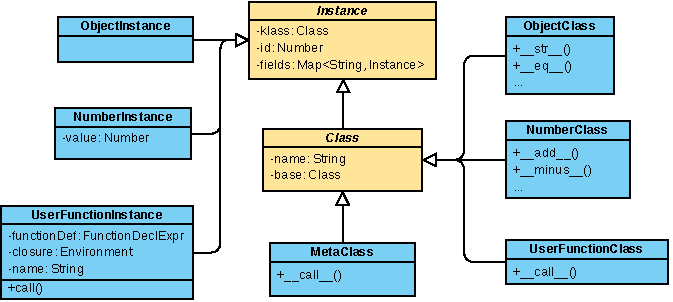
\includegraphics[width=1\textwidth]{../img/class_hierarchy}
	\label{fig:chap4:class_hierarchy}
    \caption{Class hierarchy of the object model}
\end{figure}

Classes \texttt{Instance} and \texttt{Class} are \emph{abstract}. As we can see from the Figure \ref{fig:chap4:class_hierarchy}, classes have their
respective instance classes; for example there is \texttt{NumberClass} and \texttt{NumberInstance}. This results in creating a relatively big number
of classes, but we did not find any other suitable model, because different classes of instances need to hold different value types. To illustrate this,
a \texttt{Number} need to hold a number, while \texttt{String} needs to hold a string, etc.

We could create a templated \texttt{Instance<T>} class that would have a \texttt{value: T} property. This way, we would be able to reduce the number of
classes. However, some of the instance classes also incorporate additional functionality, e.g., \texttt{UserFunctionInstance} implements a \texttt{call} method
that allows calling the function. Since there are more cases like this one, we decided to create all instances in a uniform fashion and did not go with the
generic \texttt{Instance<T>} approach.

Classes define their methods as static functions and during their initialization these methods are assigned to the class objects they represent.
A code snippet below demonstrates this:
\begin{code}
class NumberClass extends Class {
    // Overloads '+' operation of two numbers.
    static __add__(
        args: Instance[],
    ): NumberInstance {
        CheckArity(args, /* expectedArity = */ 2)
        const lhs = args[0].castOrThrow(NumberInstance)
        const rhs = args[1].castOrThrow(NumberInstance)
        return new NumberInstance(
            /* klass = */ NumberClass.get(), lhs + rhs)
    }

    constructor() {
        this.fields.set(
            /* fieldName = */ '__add__',
            new WrappedFunctionInstance(
                /* klass = */ WrappedFunctionClass.get(),
                NumberClass.__add__,
                /* functionName = */ '__add__'
            )
        )
    }
}
\end{code}

Since \texttt{NumberClass.\_\_add\_\_} is a TypeScript function it needs to be wrapped around Giflang's object. We named this wrapper a \texttt{WrappedFunctionInstance}.
The code in the actual implementation is a little more abstract since repeating this for every operation would need a lot of boilerplate.

When writing the code, we often needed the class objects, usually for instantiation. This can be seen in the code example above, e.g.,
\texttt{new NumberInstance(NumberClass.get(), lhs + rhs)}. In this case, \texttt{NumberClass.get()} is a \texttt{NumberClass} instance. Since only one
instance of each class object is needed, we used \emph{the singleton pattern}. In hindsight, it was not the best choice, because it allows changing
the interpreter state in between multiple invocations.
\begin{code}
const interpreter1 = new Interpreter()
// This code can change state of the singletons, for example
// override __add__ operation on the NumberClass.
interpreter1.visitProgramStmt(ParseGiflang('"evil" source code'))

const interpreter2 = new Interpreter()
// The second interpreter uses the same singletons and hence
// their state will be changed.
interpreter2.visitProgramStmt(ParseGiflang('source code'))
\end{code}

However, since we spawn a new WebWorker with each code run, this was not an issue. If we decide to reuse the same WebWorker, we can use a global registry
instead of singletons. Class objects in the registry can then be reinstantiated after each code execution.

\subsection{Environment state}

\subsection{Auxiliary letters}

\subsection{Code stepping (debugger)}

\subsection{Additive input}

\subsection{API}

\section{IDE}

\subsection{Choosing image format}

\subsection{State management (Redux)}

\subsection{Layout}
\chapter{Future Work}

\section{Allow language forks}

\section{Debugger with breakpoints}

\section{Improve UI}

\section{Create Challenges}

\section{Transpiler to JS/Python}

\chapter*{Conclusion}
\addcontentsline{toc}{chapter}{Conclusion}


%%% Bibliography
%%% Bibliography (literature used as a source)
%%%
%%% We employ bibTeX to construct the bibliography. It processes
%%% citations in the text (e.g., the \cite{...} macro) and looks up
%%% relevant entries in the bibliography.bib file.
%%%
%%% The \bibliographystyle command selects, which style will be used
%%% for references from the text. The argument in curly brackets is
%%% the name of the corresponding style file (*.bst). Both styles
%%% mentioned in this template are included in LaTeX distributions.

% \bibliographystyle{unsrt}    %% Author (year)
\bibliographystyle{unsrt}     %% [number]

\renewcommand{\bibname}{Bibliography}

%%% Generate the bibliography. Beware that if you cited no works,
%%% the empty list will be omitted completely.

\bibliography{bibliography}

%%% If case you prefer to write the bibliography manually (without bibTeX),
%%% you can use the following. Please follow the ISO 690 standard and
%%% citation conventions of your field of research.

% \begin{thebibliography}{99}
%
% \bibitem{lamport94}
%   {\sc Lamport,} Leslie.
%   \emph{\LaTeX: A Document Preparation System}.
%   2nd edition.
%   Massachusetts: Addison Wesley, 1994.
%   ISBN 0-201-52983-1.
%
% \end{thebibliography}


%%% Figures used in the thesis (consider if this is needed)
\listoffigures

%%% Tables used in the thesis (consider if this is needed)
%%% In mathematical theses, it could be better to move the list of tables to the beginning of the thesis.
\listoftables

%%% Abbreviations used in the thesis, if any, including their explanation
%%% In mathematical theses, it could be better to move the list of abbreviations to the beginning of the thesis.
\chapwithtoc{List of Abbreviations}

%%% Attachments to the bachelor thesis, if any. Each attachment must be
%%% referred to at least once from the text of the thesis. Attachments
%%% are numbered.
%%%
%%% The printed version should preferably contain attachments, which can be
%%% read (additional tables and charts, supplementary text, examples of
%%% program output, etc.). The electronic version is more suited for attachments
%%% which will likely be used in an electronic form rather than read (program
%%% source code, data files, interactive charts, etc.). Electronic attachments
%%% should be uploaded to SIS and optionally also included in the thesis on a~CD/DVD.
%%% Allowed file formats are specified in provision of the rector no. 72/2017.
\appendix
\chapter{Attachments}

\section{First Attachment}

\openright
\end{document}
